\documentclass[10pt,a4paper]{article}
\usepackage[margin=2cm]{geometry}
\usepackage{amsmath,amssymb}
\usepackage{graphicx}
\usepackage{booktabs}
\usepackage{xcolor}
\usepackage{caption}
\usepackage{float}
\usepackage[colorlinks=true,linkcolor=black,citecolor=black,urlcolor=blue]{hyperref}
\captionsetup{font=small,labelfont=bf}
\graphicspath{{../figures/}{../demo/out/}}
\newcommand{\Pret}{P_{\mathrm{ret}}}

\title{\textbf{From Memorization to Generalization}\\[2pt]
\large Interference, False Memories, Forgetting and Robustness in Classical and Modern Hopfield Networks\\[2pt]
\normalsize INCM 2026 $\cdot$ Project 15: Associative Memory with Hopfield Networks $\cdot$ Final report}
\author{Athmeeya M Kashyap (2024113015) \and Laksh Mittal (2024113003)}
\date{}

\begin{document}
\maketitle

\begin{abstract}
We model how the form of a network's energy function decides whether it recalls individual memories,
blends them, recalls a prototype it never stored, or forgets. Four model families (classical Hebbian/Storkey,
dense polynomial and exponential, continuous exponential = one attention head, and a two-layer
feature/memory-neuron circuit) were implemented from scratch and compared on identical patterns and
cues at finite $N$, with 50 independent pattern sets $\times$ 20 cues per condition. All six pre-specified
primary tests support their hypotheses after Holm correction (Table~\ref{tab:primary}).
Capacity exponents match theory ($1.92$ and $3.08$ for $n=3,4$; exponential rate $0.34$ per neuron).
As similar memories accumulate, every finite-order model switches from recalling stored items to recalling
their unstored prototype, and the crossover load $P^*$ grows with interaction order (e.g.\ at $c=0.4$:
$8$, $29$, $131$ memories per prototype for $n=2,3,4$; never for the exponential model): a DRM-like false
memory whose rate rises with the number of associates. Lower $\beta$ or higher temperature produces blending and prototype
recall. Deleting memory neurons in the two-layer circuit destroys memories all-or-none (concept-cell
signature), unlike graded synaptic loss in the classical network. The same interference governs a single
attention head and real GPT-2 keys. Bounded/decaying synapses turn catastrophic overload into a recency
gradient with a span of $\approx0.05N$. Several secondary predictions did not hold, and we report them as found.
\end{abstract}

%=====================================================================
\section{Aim and questions}
Human memory is content addressable; Hopfield networks~\cite{hopfield82} make recall a relaxation into
an energy minimum. The classical network stores only $\approx0.138N$ random patterns~\cite{amit85,amit87}
and similar memories interfere~\cite{fontanari90}. Dense and exponential associative memories~\cite{krotov16,demircigil17}
raise capacity to polynomial or exponential in $N$. Their update is transformer attention~\cite{ramsauer21}.
They can be built from two-layer circuits~\cite{krotov21}, and with many similar memories they generalise to
unstored prototypes~\cite{ambrogioni24,pham25}.

\textbf{Research question.} How does the energy function (classical, dense, exponential) change retrieval under
memory load, similarity, cue corruption and continual storage, and when does recall of individual memories give way to
recall of their shared prototype? The hypotheses H1--H6 are those of the proposal and are restated with
their results in Table~\ref{tab:primary}.

%=====================================================================
\section{Models, data and protocol}
\paragraph{Data.} All memories are synthetic and seeded (NumPy \texttt{SeedSequence} from one master seed,
addressed by experiment/condition/set). \emph{Random memories}: $\xi_i^\mu=\pm1$. \emph{Prototype-structured}:
$K$ unstored prototypes $\zeta^k$; each memory copies one and flips each bit with probability $(1-c)/2$,
giving expected overlap $c$ with its prototype and $c^2$ with siblings (verified numerically in the tests).
\emph{Cues}: exactly $\mathrm{round}(\eta N)$ bits of a stored memory flipped (initial overlap $1-2\eta$), or a
corrupted prototype (the DRM lure).

\paragraph{Models.}
\textbf{M1} classical: $E=-\tfrac12\sum_{i\ne j}W_{ij}s_is_j$ with Hebbian or Storkey~\cite{storkey97} weights.
\textbf{M2} dense: $E=-\sum_\mu F(\xi^\mu\!\cdot s)$, $F(x)=x^n$ ($n=2,3,4$) or $e^x$; each neuron takes the sign
with lower energy (eq.~2 of the proposal); the exponential model is computed in log space.
\textbf{M3} continuous exponential: $x\leftarrow X\,\mathrm{softmax}(\beta X^\top x)$~\cite{ramsauer21}.
\textbf{M4} two-layer~\cite{krotov21}: feature neurons $v$ and memory neurons $h_\mu=\sum_iW_{i\mu}v_i$ with
pairwise synapses only; $v_i\leftarrow\mathrm{sgn}\sum_\mu W_{i\mu}f_\mu$ with $f_\mu=g_\mu F'(h_\mu)$ ($F=h^4$)
or $f=\mathrm{softmax}(\beta h+\log g)$. Its Lyapunov function is $E=-\sum_\mu g_\mu F(h_\mu)$, or $-\beta^{-1}\log\sum_\mu g_\mu e^{\beta h_\mu}$
for the softmax. Convexity of $F$ makes $E$ non-increasing even after lesions. Each memory neuron
(strength $g_\mu$) can be lesioned, and with decaying strengths it forgets.

\paragraph{Dynamics, noise, forgetting.} Asynchronous updates in a fresh random order, one sweep $=N$ updates,
stop at a fixed point or after 50 sweeps (M3: synchronous, until $\max|\Delta x|<10^{-6}$ or 50 iterations).
Glauber noise $P(s_i=+1)=1/(1+e^{-\Delta E_i/T})$~\cite{glauber63}, where $\Delta E_i=2h_i$ in M1. The polynomial energy is scaled by
$1/(2N^{n-1})$, so $n=2$ equals M1 exactly, and the exponential model uses the log-sum-exp energy. A Glauber run
(50 sweeps) is followed by a $T=0$ quench to classify the basin it ended in. Forgetting: clipping
$W\leftarrow\mathrm{clip}(W+\xi\xi^\top/N,\pm A/\sqrt N)$~\cite{parisi86} or decay $W\leftarrow\lambda W+\xi\xi^\top/N$~\cite{nadal86,mezard86};
in M4, $g_\mu\leftarrow\lambda g_\mu$ at each new memory.
\textit{Implementation:} Python/NumPy/Numba, own simulator, no Hopfield libraries; experiments were run as Kaggle CPU jobs.

\paragraph{Metrics and statistics.} $\Pret=\Pr[m_{\mathrm{final}}\ge0.95]$ (also 0.90/0.99). Final states are classified, in order, as
\emph{target} ($m\ge0.95$ with the cued memory), \emph{other memory}, \emph{prototype} ($m\ge0.95$ with the binarised state), or
\emph{spurious}. For M3, memory overlaps use the raw state, so a continuous blend is not a memory, and ``spurious'' means a blend. Each
condition uses 50 pattern sets $\times$ 20 cues (E5a: 10 memories $\times$ 4 cues; E7: every one of 600 memories).
Cue outcomes are averaged within a set; we report means with 95\% percentile bootstrap CIs over sets (2000 resamples).
Model comparisons are paired (identical patterns, cues and update orders). Each hypothesis has one pre-specified
primary test, Holm-corrected; everything else is exploratory.

\paragraph{Correctness checks (all passed).} (i) $E$ never increased in any recorded run of any model, including
lesioned/noisy M4 and Storkey/clipped/decayed M1 (0 violations in Part A's 240\,000 recalls). (ii) All stored patterns are exact fixed
points at $\alpha=0.02$ for every model, N, and rule. (iii) Hebbian $\alpha_c$: see Part A. (iv) M2 with $n=2$ reproduces
M1 \emph{update by update} (same states, trajectories, recall times; energies equal up to the constant $-P/2$), at $T=0$ and $T=0.4$.
Also: Storkey matches a brute-force reference implementation. These are the 14 unit tests in \texttt{tests/}.

%=====================================================================
\section{Results}
\subsection*{Part A: validation of the classical model (checks, not findings)}
\begin{figure}[H]\centering
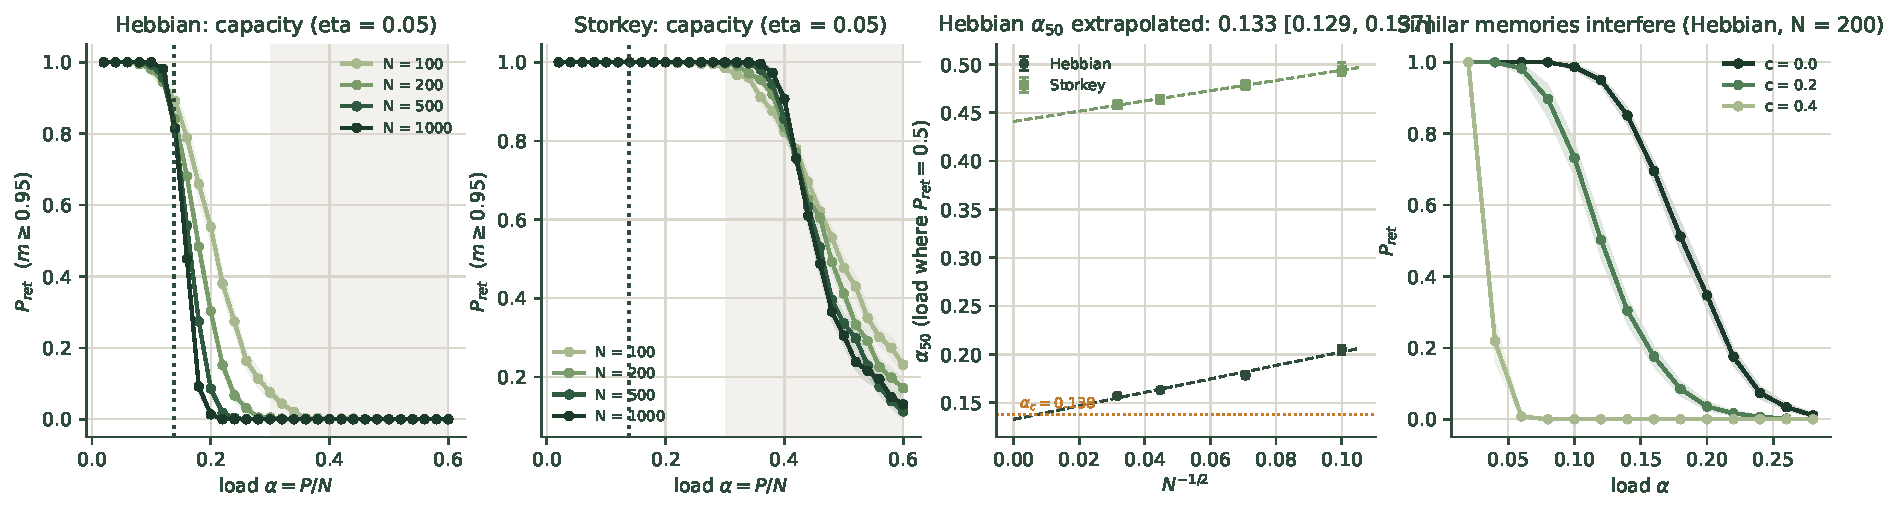
\includegraphics[width=\linewidth]{partA_capacity.pdf}
\caption{Part A. Retrieval vs load for Hebbian and Storkey networks ($\eta=0.05$; shaded: beyond the proposal's 0.30 range,
added so the Storkey transition is inside the grid). Third panel: load $\alpha_{50}$ at which $\Pret=0.5$, extrapolated in $N^{-1/2}$.
Right: similar memories interfere (reproduces the deck pilot with 50 sets).}
\label{fig:partA}\end{figure}
The transition sharpens with $N$, as expected. The Hebbian $\alpha_{50}$ is $0.205,\,0.178,\,0.163,\,0.157$ for $N=100$--$1000$.
Extrapolated linearly in $N^{-1/2}$ it gives $\alpha_\infty=0.133$ [0.129, 0.137]; the sensitivity fit in $N^{-1}$ gives $0.152$.
The theoretical $0.138$ lies between the two extrapolations, just outside the CI of the pre-chosen one, so check (iii) is satisfied
only up to the uncertainty in the finite-size scaling form. Storkey learning roughly triples capacity ($\alpha_\infty=0.441$
[0.434, 0.447]) and tolerates more cue noise ($\eta_{50}=0.383$ vs $0.317$ at $\alpha=0.1$; $0.427$ vs $0.413$ at $0.05$).
Similarity is very damaging: at $N=200$, $\alpha_{50}$ falls from $0.181$ ($c=0$) to $0.120$ ($c=0.2$) and $0.033$ ($c=0.4$).

\subsection*{E1: capacity across models (H1)}
\begin{figure}[H]\centering
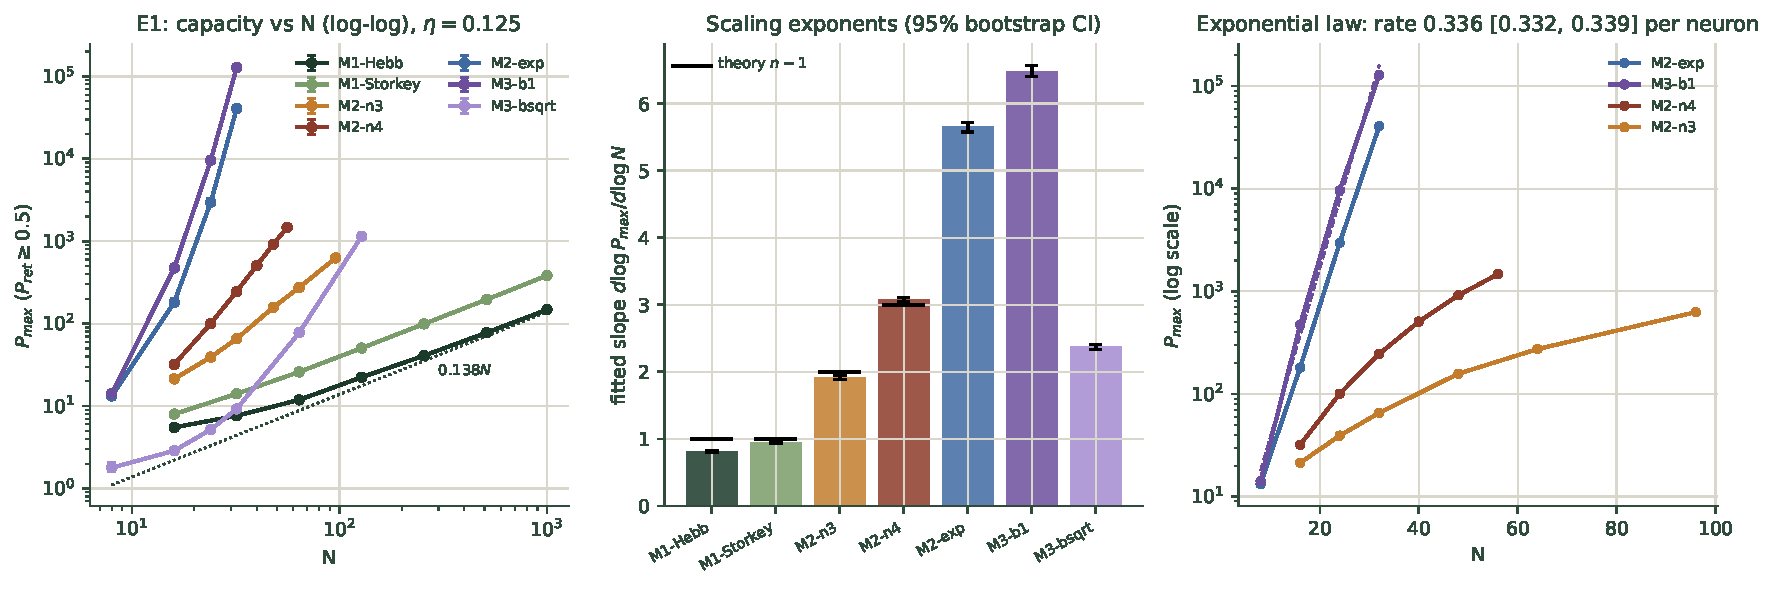
\includegraphics[width=\linewidth]{e1_capacity.pdf}
\caption{E1. $P_{\max}$ (largest $P$ with $\Pret\ge0.5$, $\eta=0.125$) on identical patterns and cues; fitted log-log slopes with
95\% bootstrap CIs vs theory $n-1$; exponential models on a log-linear scale.}
\label{fig:e1}\end{figure}
Scaling exponents: M2 $n=3$: $1.92$ [1.89, 1.94]; $n=4$: $3.08$ [3.04, 3.11], close to $N^{n-1}$ (the small deficit for $n=3$
matches the expected $1/\log N$ correction). M1 Hebbian: $0.81$ [0.80, 0.83] over $N=16$--$1000$, approaching $1$ at large $N$
(the slope between 256 and 1000 is 0.94; $P_{\max}/N=0.147$ at $N=1000$). Storkey: $0.94$. The exponential model grows as
$e^{0.336N}$ [0.332, 0.339], and M3 with $\beta=1$ as $e^{0.379N}$. Both are below the trivial $\ln 2$ ceiling. They are above
Demircigil et al.'s rate bound for retrieval of \emph{all} patterns under noise $\rho=0.125$ ($0.158$), which uses a stricter
criterion and is asymptotic. M3 with attention scaling $\beta=1/\sqrt N$ grows faster than any polynomial but much more slowly than $\beta=1$.
\textbf{Primary test (H1):} slope(M2 $n=4$) $-$ slope(M1) $=2.27$ [2.23, 2.30], $p<0.001$. \textbf{Supported.}

\subsection*{E2: memorization to generalization (H2, main experiment)}
\begin{figure}[H]\centering
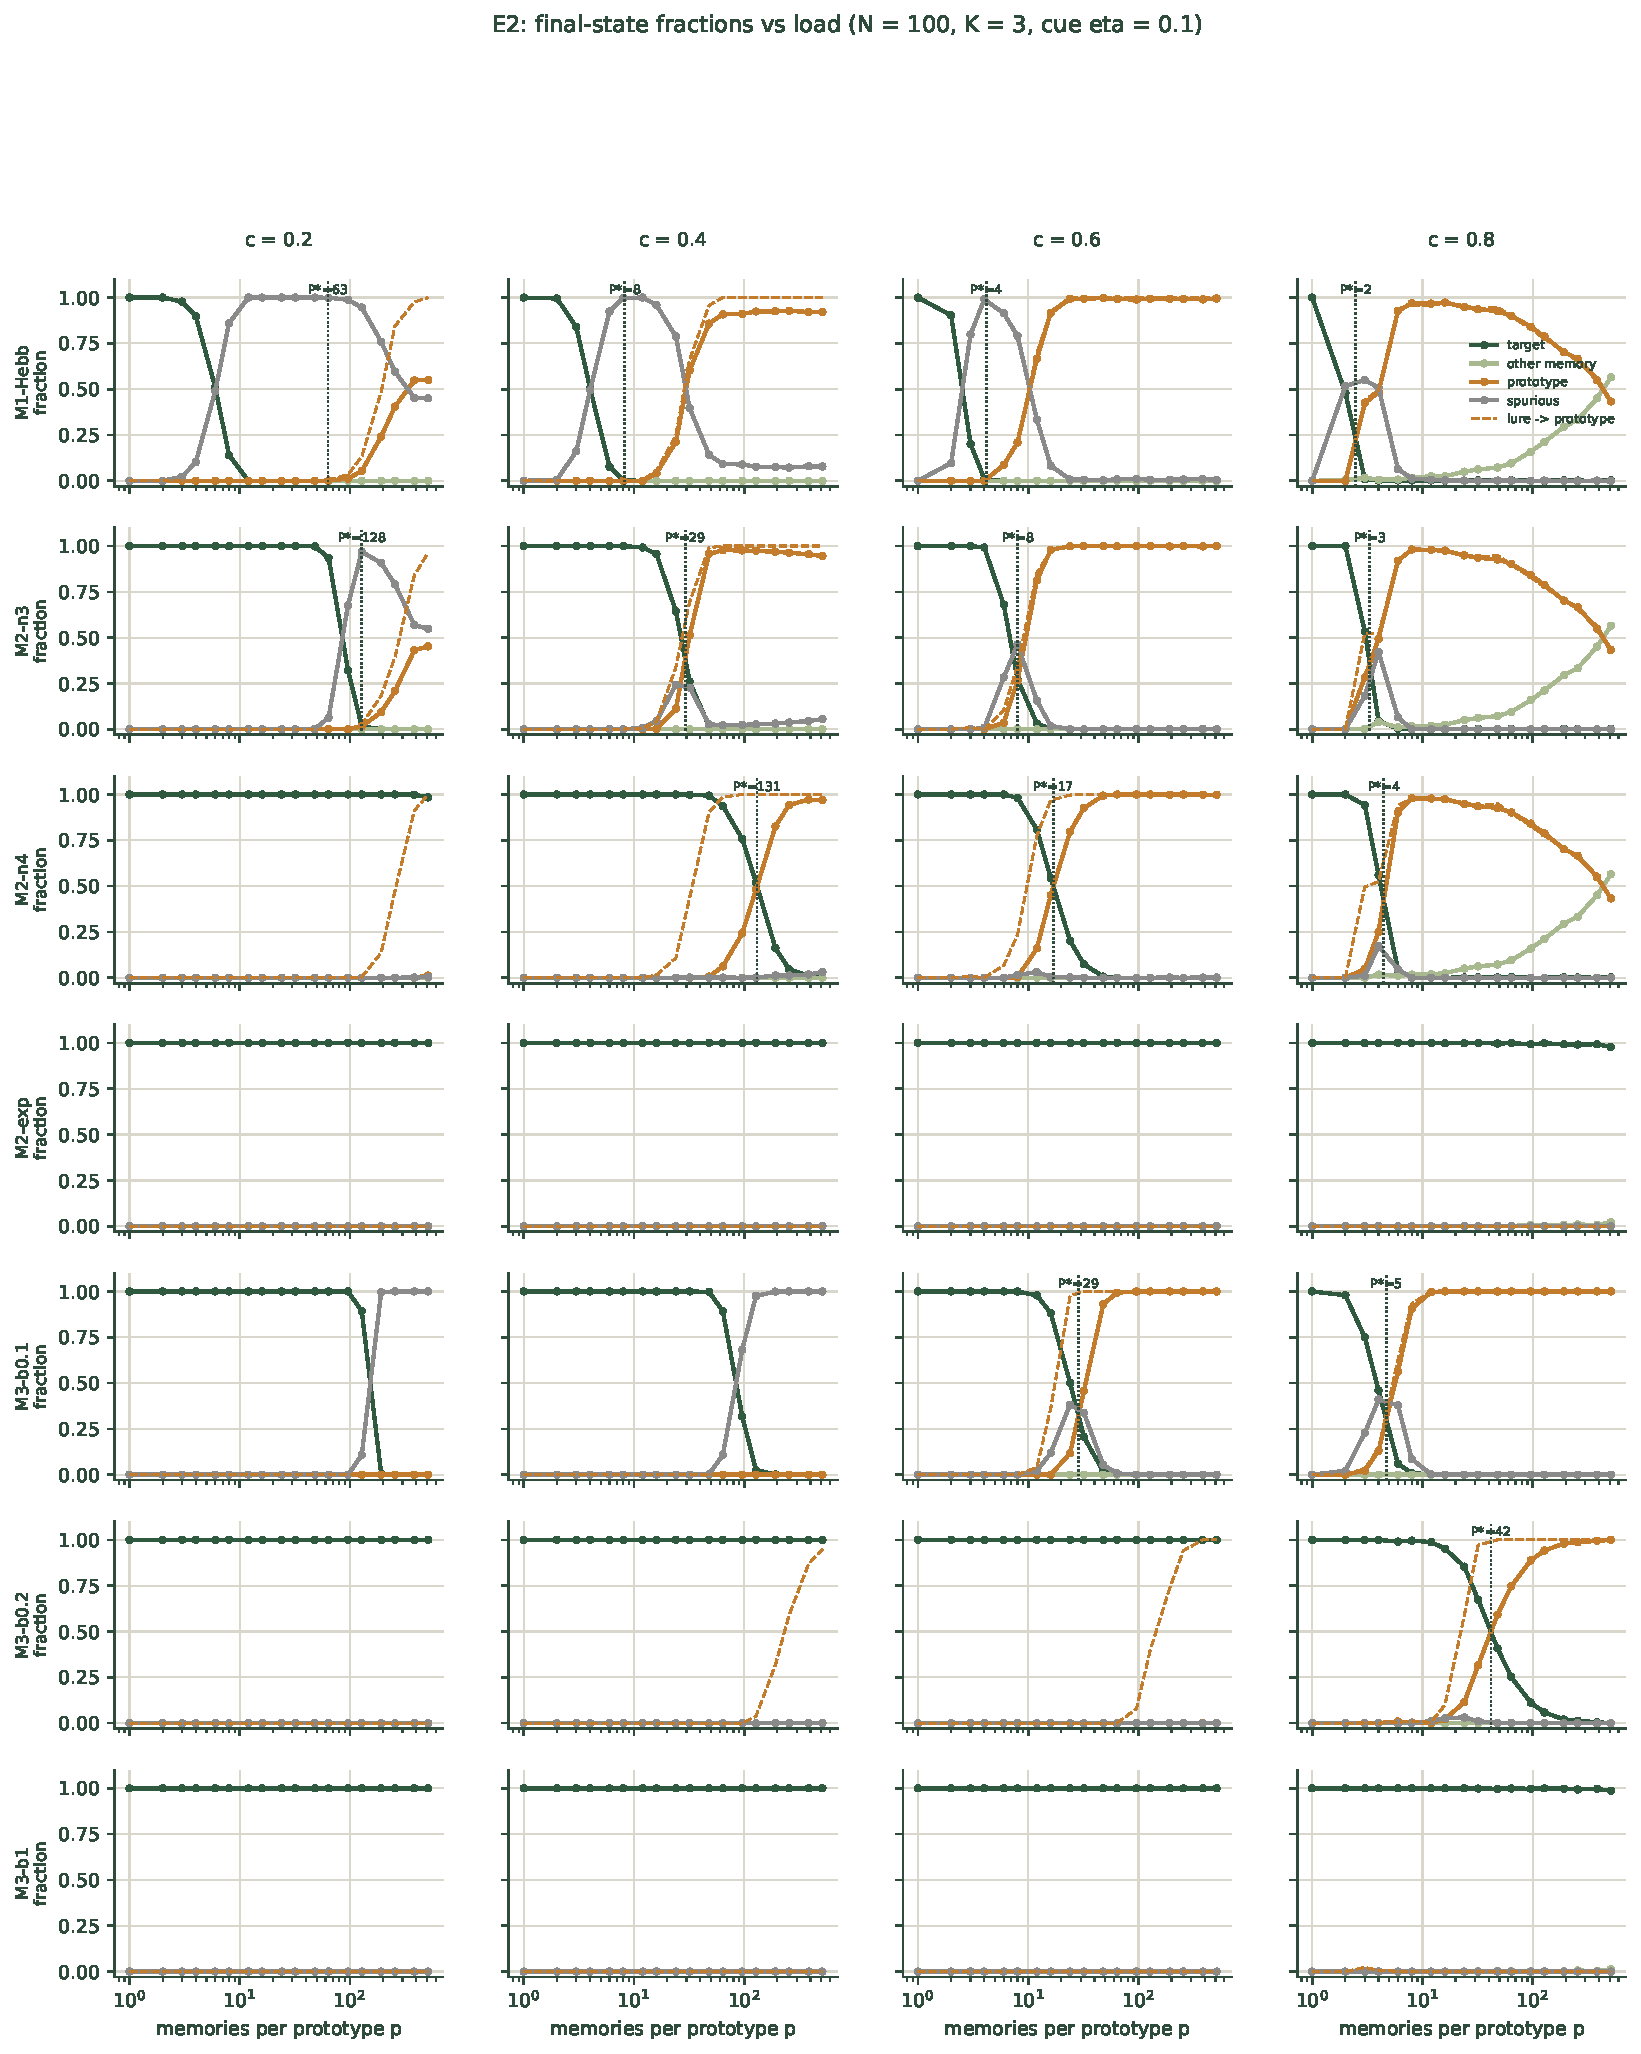
\includegraphics[width=0.92\linewidth]{e2_state_fractions.pdf}
\caption{E2. Fractions of final states for memory cues vs memories per prototype $p$ ($N=100$, $K=3$, $\eta=0.1$). Dashed:
recall of the prototype from a corrupted-prototype (lure) cue. Dotted line: crossover $P^*$.}
\label{fig:e2}\end{figure}
\begin{figure}[H]\centering
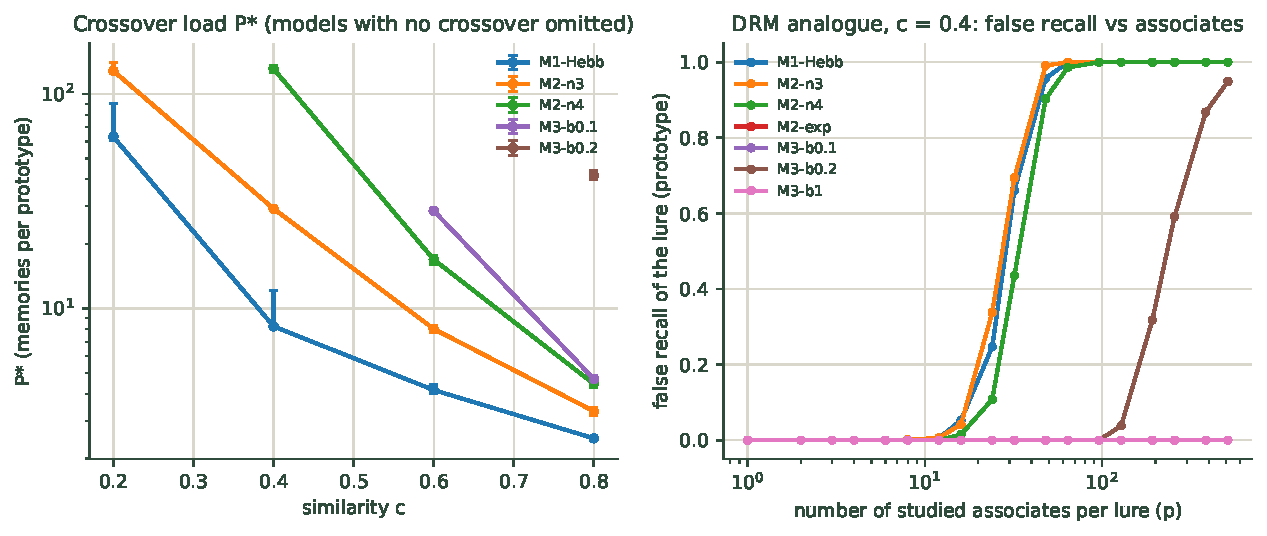
\includegraphics[width=0.85\linewidth]{e2_pstar_drm.pdf}
\caption{Left: crossover load $P^*$ vs similarity (censored models omitted). Right: false recall of the unstudied lure rises with the
number of studied associates, as in DRM~\cite{roediger95,robinson97}.}
\label{fig:e2b}\end{figure}
\begin{table}[H]\centering\small
\begin{tabular}{lcccc}\toprule
$P^*$ (memories per prototype) & $c=0.2$ & $c=0.4$ & $c=0.6$ & $c=0.8$\\\midrule
M1 Hebbian & 63 [61, 90] & 8.3 [8.1, 12.2] & 4.2 [4.0, 4.4] & 2.5 [2.4, 2.5]\\
M2 $n=3$ & 128 [125, 140] & 29 [29, 30] & 8.0 [7.8, 8.4] & 3.3 [3.2, 3.5]\\
M2 $n=4$ & $>512$ & 131 [126, 135] & 17 [16, 18] & 4.5 [4.3, 4.6]\\
M2 exponential & $>512$ & $>512$ & $>512$ & $>512$\\
M3 $\beta=0.1$ / $0.2$ / $1$ & $>512$ & $>512$ & 29 / $>512$ / $>512$ & 4.7 / 42 / $>512$\\\bottomrule
\end{tabular}
\caption{Crossover loads (95\% bootstrap CI). $>512$: prototype never overtook the target within the grid.}
\label{tab:pstar}\end{table}
Every finite-order model switches from item recall to recall of the never-stored prototype. $P^*$ falls steeply with $c$ and
rises with interaction order, so higher-order models stay in the memorization regime longer. The exponential model ($N=100$)
and M3 at large $\beta$ never switch in range (their transition is expected at exponentially large $P$~\cite{pham25}).
Lure cues converge to the prototype with a probability that rises with the number of associates (Fig.~\ref{fig:e2b}). This is the
signature of DRM false recall. In M1 at low $c$ the item regime ends in spurious mixtures before the prototype regime begins
(e.g.\ $c=0.2$), so ``loss of items'' and ``gain of the prototype'' are distinct transitions in the classical network.
\textbf{Primary test (H2):} $\log P^*(n=3)-\log P^*(\mathrm{M1})$ at $c=0.4$: $1.26$ [0.87, 1.30] (ratio 3.5), $p<0.001$. \textbf{Supported.}

\subsection*{E3: blending, $\beta$ and temperature (H3)}
\begin{figure}[H]\centering
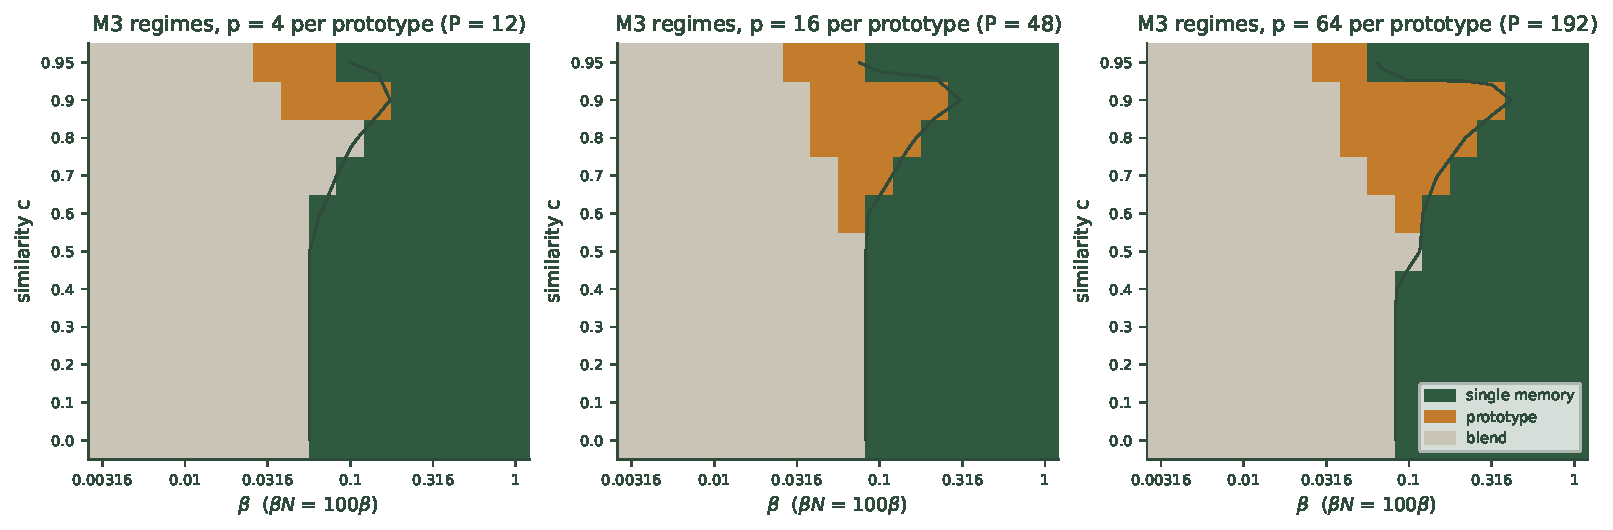
\includegraphics[width=\linewidth]{e3_m3_regime_map.pdf}
\caption{E3. Dominant final state of M3 in the $(\beta,c)$ plane for 4, 16 and 64 memories per prototype ($N=100$, $K=3$). Line:
50\% single-memory contour.}
\label{fig:e3}\end{figure}
\begin{figure}[H]\centering
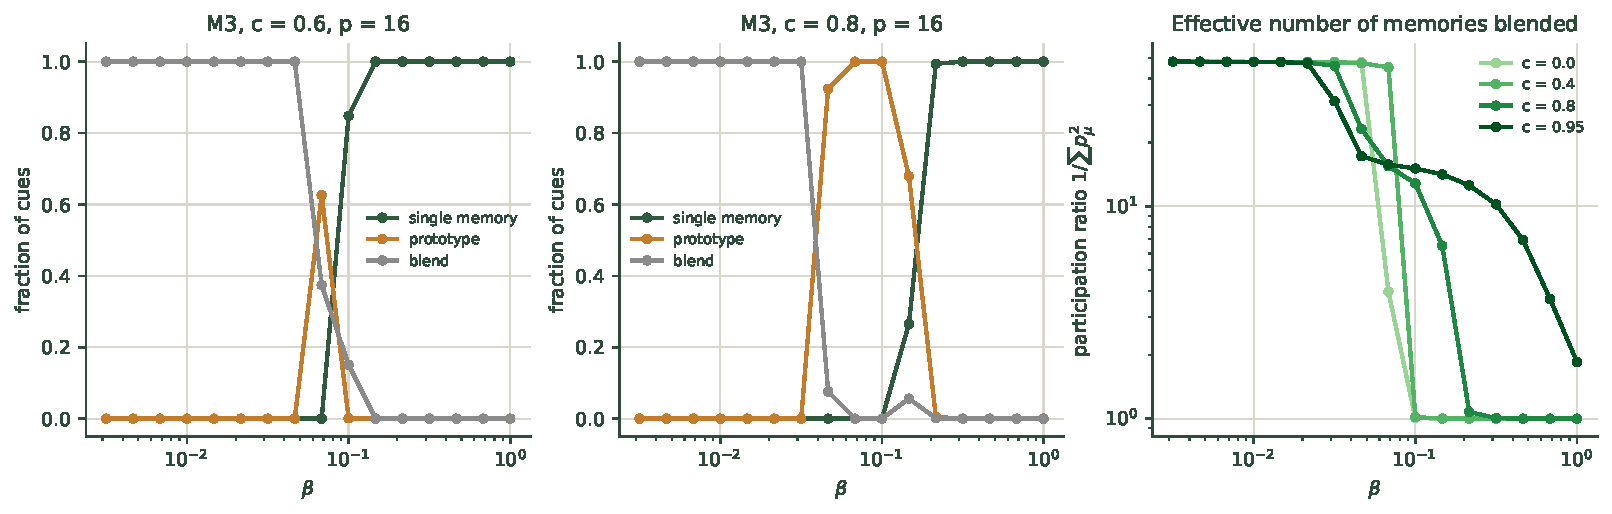
\includegraphics[width=\linewidth]{e3_m3_fractions.pdf}
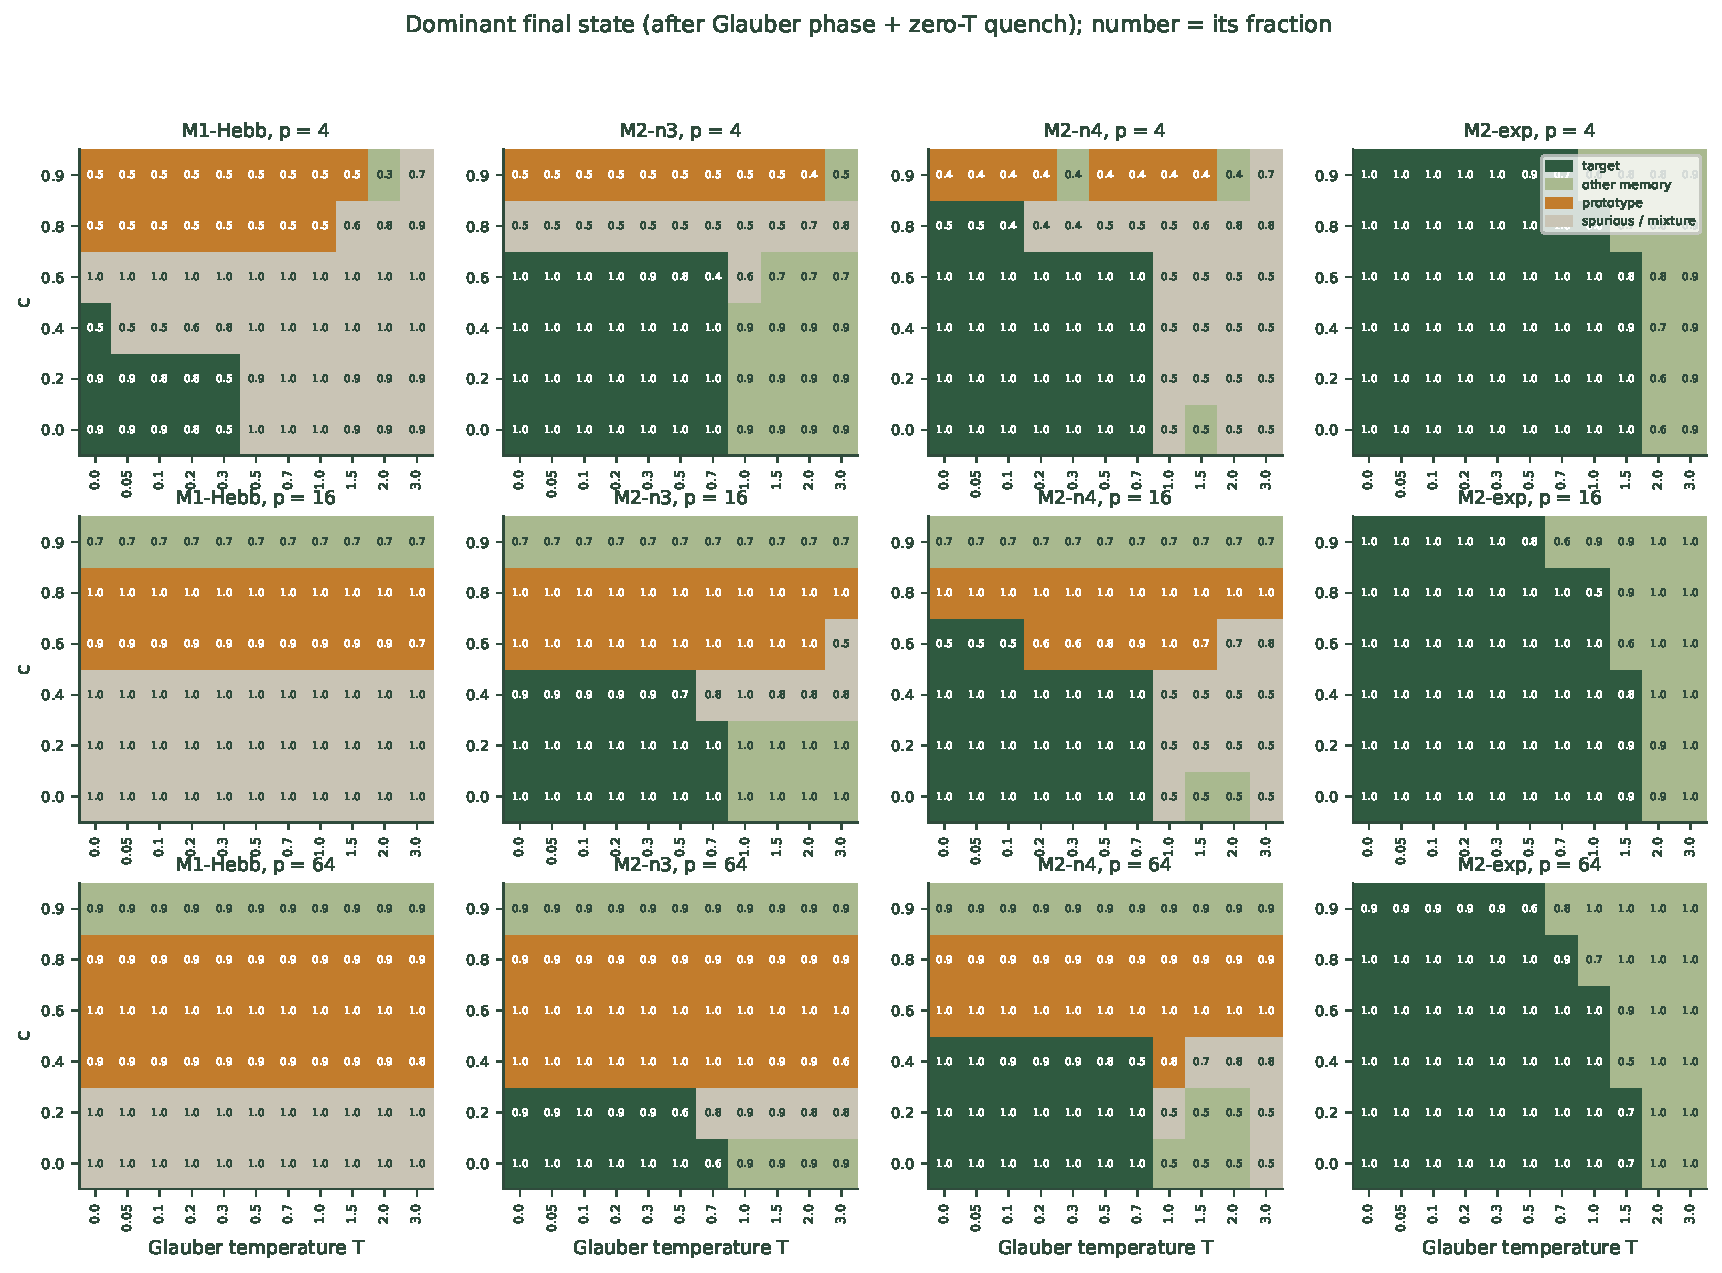
\includegraphics[width=\linewidth]{e3_glauber_maps.pdf}
\caption{Top: regime fractions and participation ratio (number of memories blended) vs $\beta$. Bottom: binary models with
Glauber temperature $T$ (dominant quenched state; number = its fraction).}
\label{fig:e3b}\end{figure}
M3 shows three regimes. High $\beta$ gives single-memory recall. Low $\beta$ gives a global blend: the participation ratio approaches $P$.
Intermediate $\beta$ at high similarity gives prototype recall. The prototype region exists only for $c\gtrsim0.55$ and widens with
load ($p=4\to64$). The single-recall boundary is at $\beta\approx0.083$ ($\beta N\approx8$) for $c\le0.5$ and moves to larger $\beta$
as $c$ grows ($0.12$, $0.17$, $0.31$ at $c=0.7,0.8,0.9$). The switch between regimes is abrupt along $\beta$ (Fig.~\ref{fig:e3b}), mirroring gist-over-verbatim recall.
In the binary models, temperature plays the same role where a prototype attractor exists: in M2 $n=4$ ($c=0.6$, $p=16$) prototype recall rises from
0.46 at $T=0$ to 0.97 at $T=1$ while target recall falls. M1 at the same loads is already in the prototype or spurious regime,
and very high $T$ destroys all retrieval.
\textbf{Moderate noise did not help} escape wrong attractors: for random memories near capacity (Fig.~\ref{fig:e3c}),
the best $T>0$ changed $\Pret$ by $-0.002$ to $+0.012$, with every CI including 0 (M1 at $N=200$; M2 $n=3$ at $N=64$).
\textbf{Primary test (H3):} M3 ($p=16$, $c=0.6$), per-set Spearman($\beta$, single-recall fraction): median $\rho=0.88$, Wilcoxon $p=1.6\times10^{-11}$. \textbf{Supported.}

\begin{figure}[H]\centering
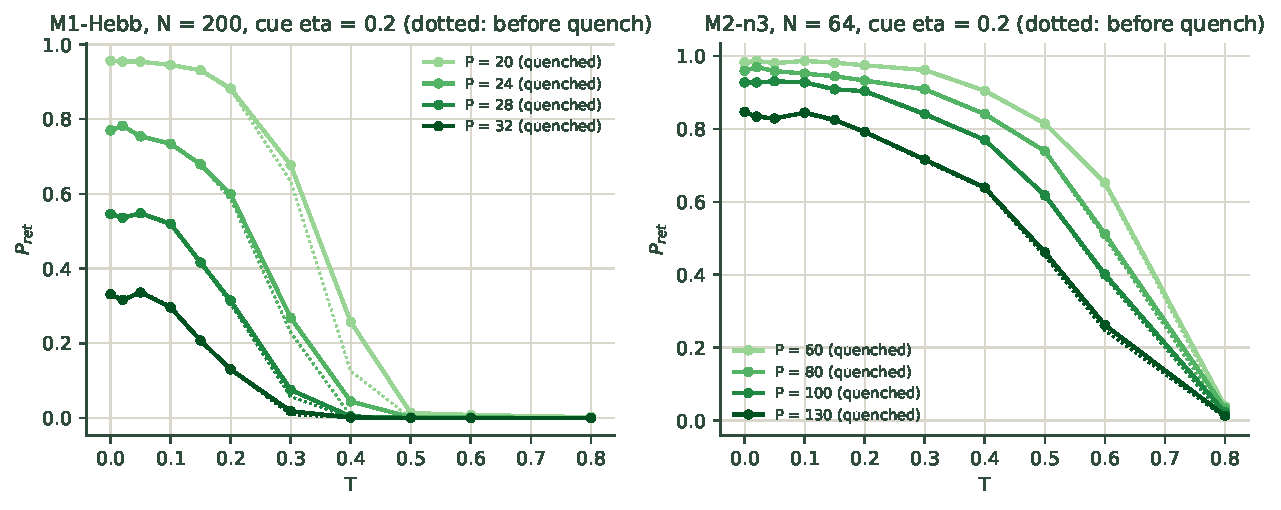
\includegraphics[width=0.75\linewidth]{e3_noise_escape.pdf}
\caption{E3c. Retrieval vs Glauber temperature for random memories near capacity (solid: after quench; dotted: noisy state before quench).}
\label{fig:e3c}\end{figure}

\subsection*{E4: recovery dynamics and recall time}
\begin{figure}[H]\centering
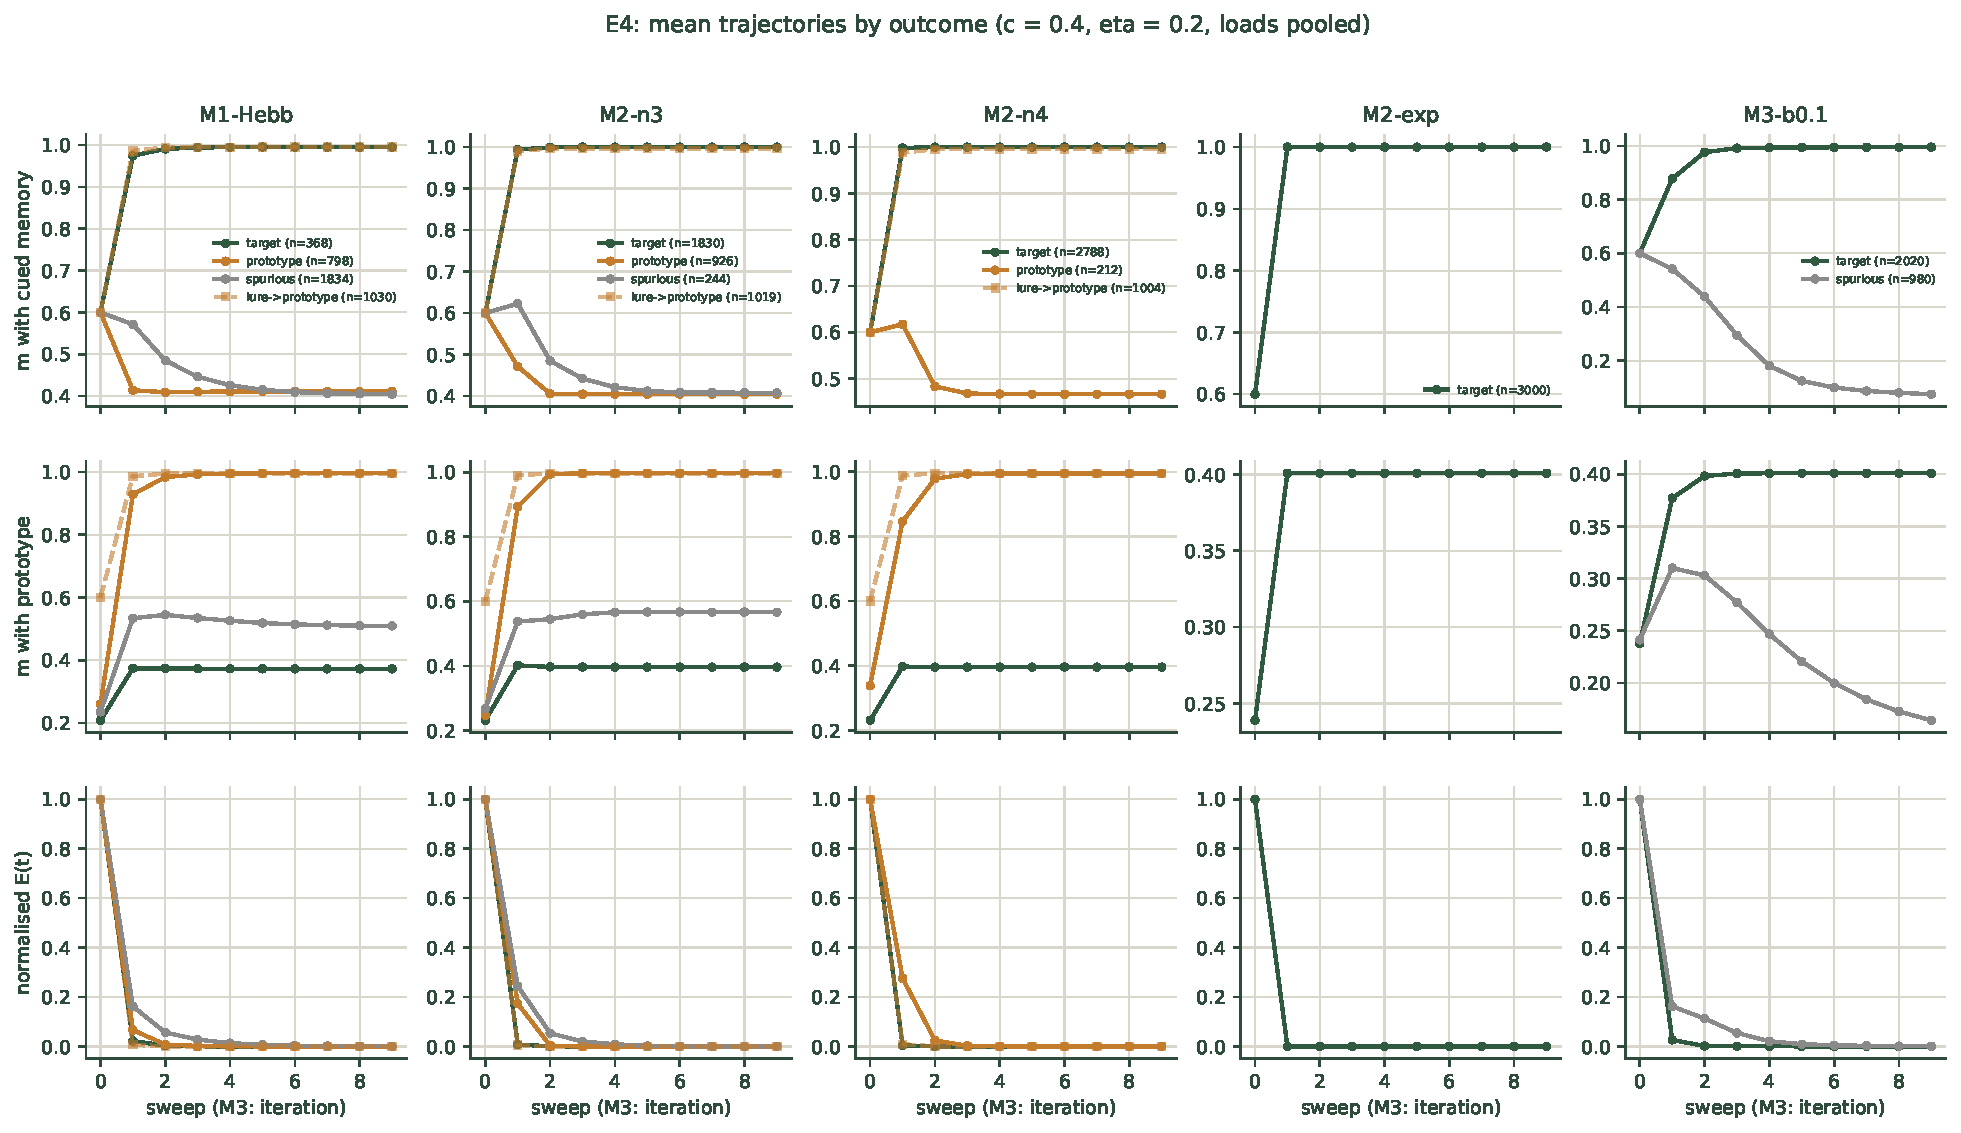
\includegraphics[width=\linewidth]{e4_trajectories.pdf}
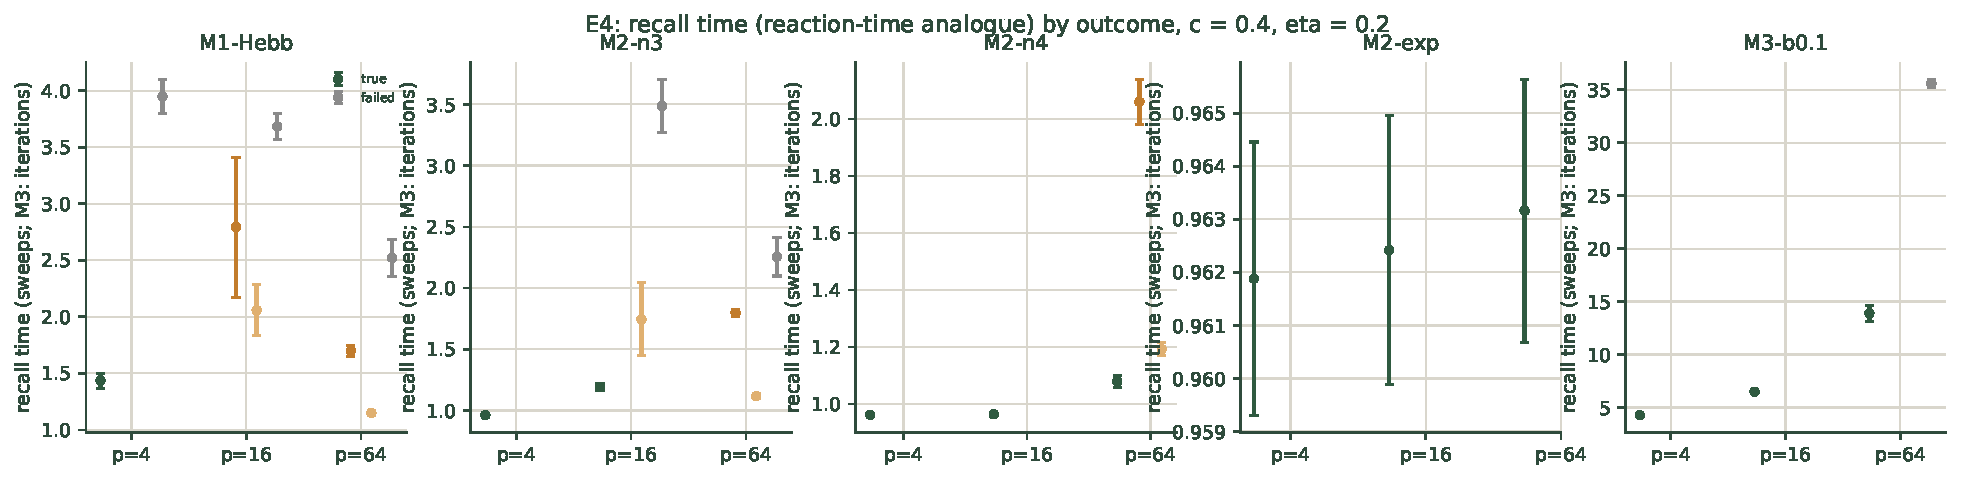
\includegraphics[width=\linewidth]{e4_recall_time.pdf}
\caption{E4 ($c=0.4$, $\eta=0.2$). Top: mean $m(t)$ with the cued memory and with its prototype, and normalised $E(t)$, by outcome.
Bottom: recall time (sweeps to the last flip) by outcome and load.}
\label{fig:e4}\end{figure}
True recalls converge within about one sweep. In false recalls the overlap with the cued memory drops within the first sweep
(to $\approx0.41$ in M1 and $n=3$; in $n=4$ it first rises slightly, $0.60\to0.62$, then falls), while the overlap with the prototype climbs to 1 over
1--2 sweeps. Failed (spurious) recalls are slowest to settle. In M2 $n=4$ at $p=64$, where true and false recalls
co-occur in all 50 sets, false recalls from memory cues took $+0.98$ sweeps longer than true recalls (paired Wilcoxon $p=1.8\times10^{-15}$).
False recalls from lure cues took $+0.11$ sweeps longer ($p=7\times10^{-6}$). In M1 and $n=3$ at high load, lure$\to$prototype recall
(1.1--1.2 sweeps) is faster than memory-cue$\to$prototype recall (1.7--1.8). So false memories are slower than true ones
when both start equally far away, but a lure that is already close to the gist is recalled quickly. Recall time of true recalls rises with $\eta$ in M1, M2 ($n=3,4$, exp). The false-recall time rises with $\eta$ in M1 and $n=3$ but falls in $n=4$,
and M3 is non-monotone (Fig.~\ref{fig:e4b}). Caveat: recall times are confounded with cue distance; these comparisons are exploratory.

\begin{figure}[H]\centering
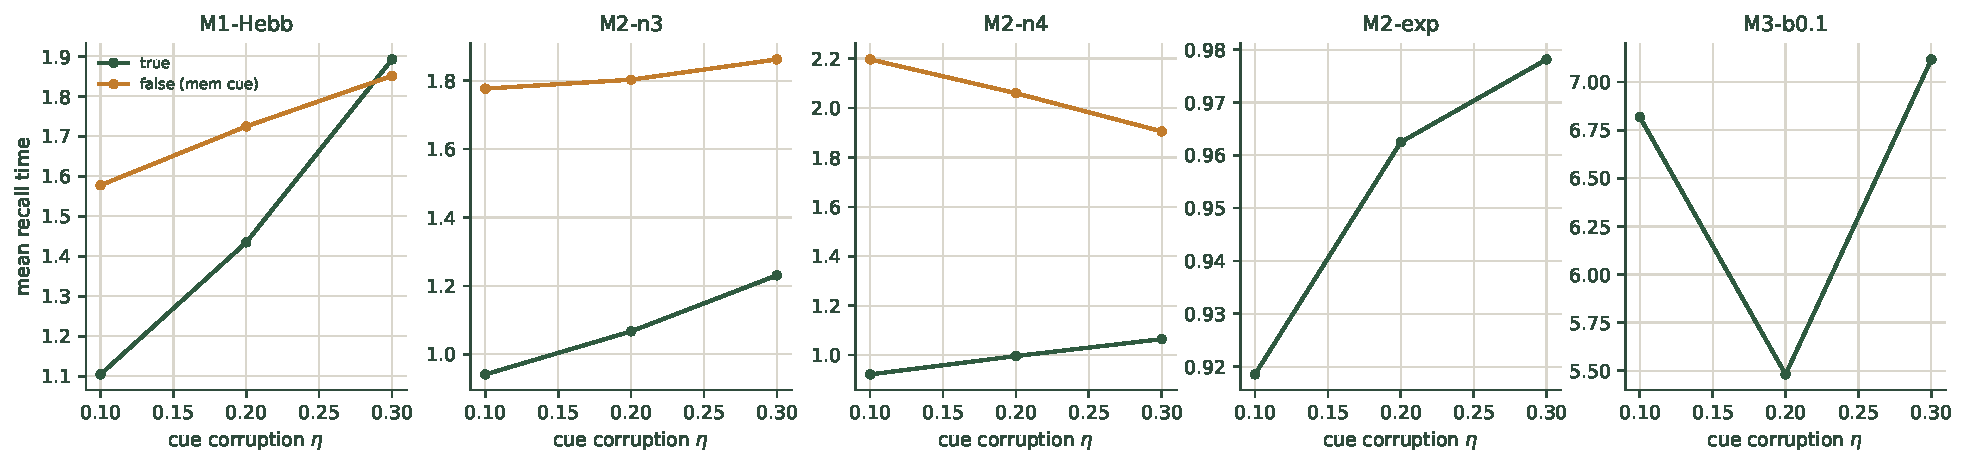
\includegraphics[width=\linewidth]{e4_time_vs_eta.pdf}
\caption{E4. Mean recall time vs cue corruption for true and false (memory-cue $\to$ prototype) recalls, $c=0.4$, loads pooled.}
\label{fig:e4b}\end{figure}

\subsection*{E5: lesions and concept cells (H4)}
\begin{figure}[H]\centering
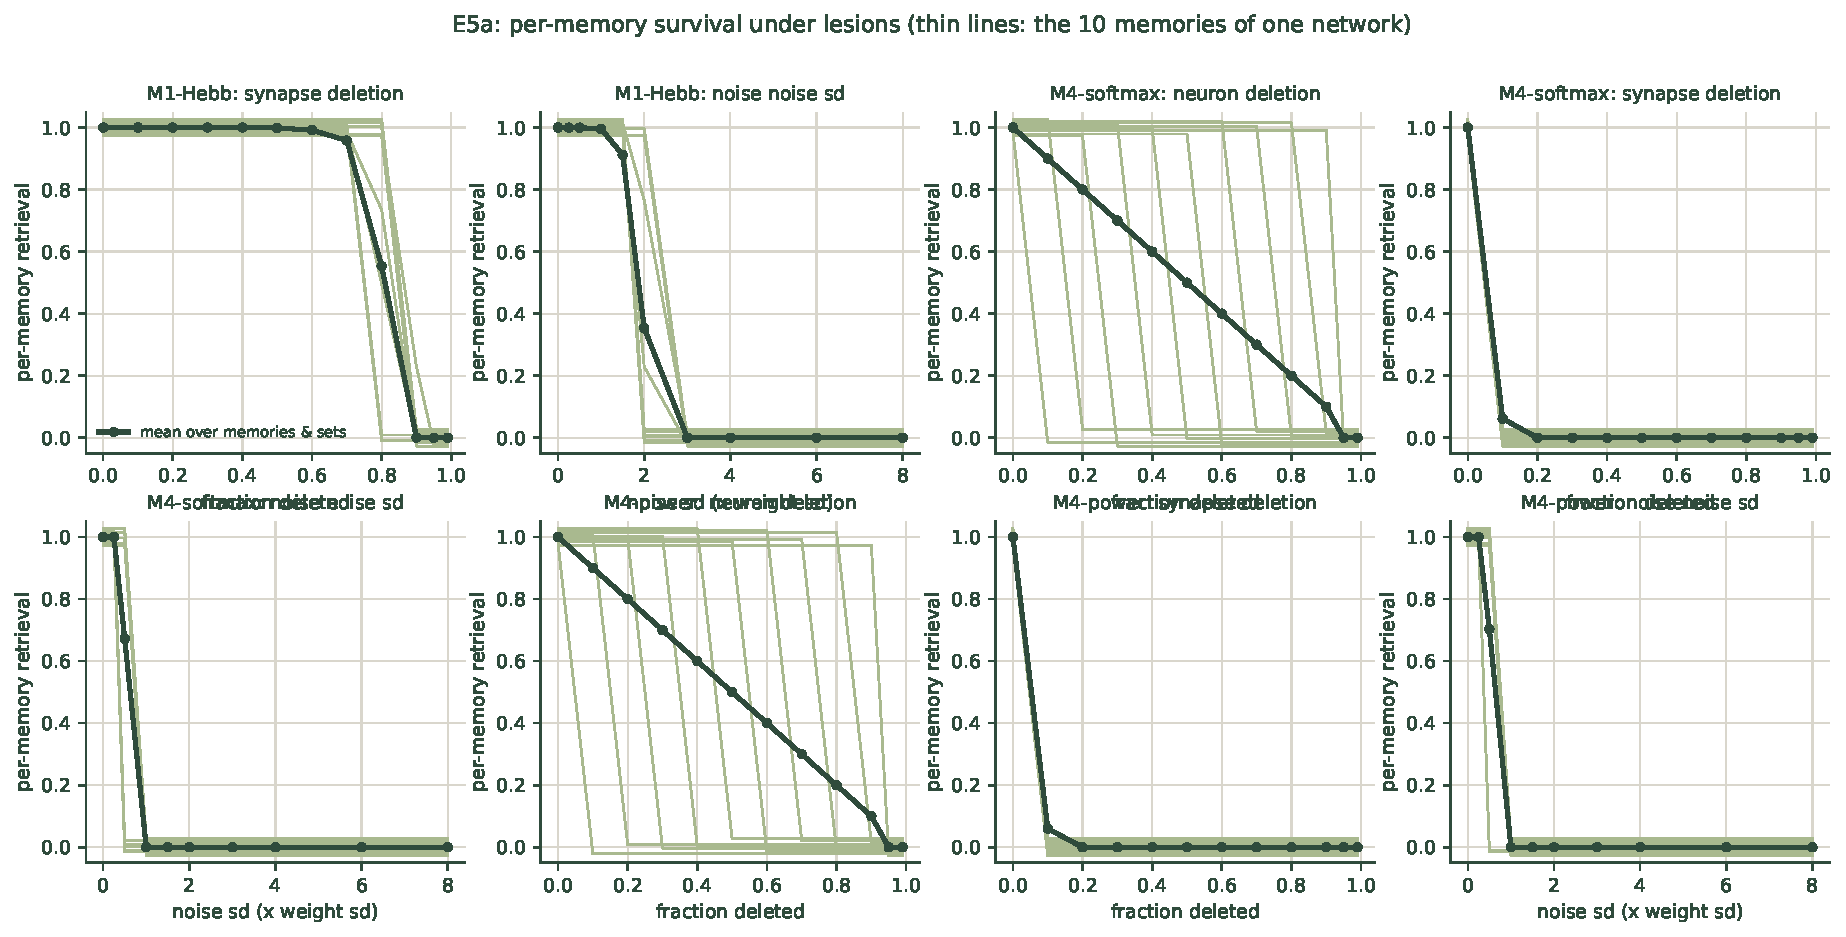
\includegraphics[width=\linewidth]{e5_survival.pdf}
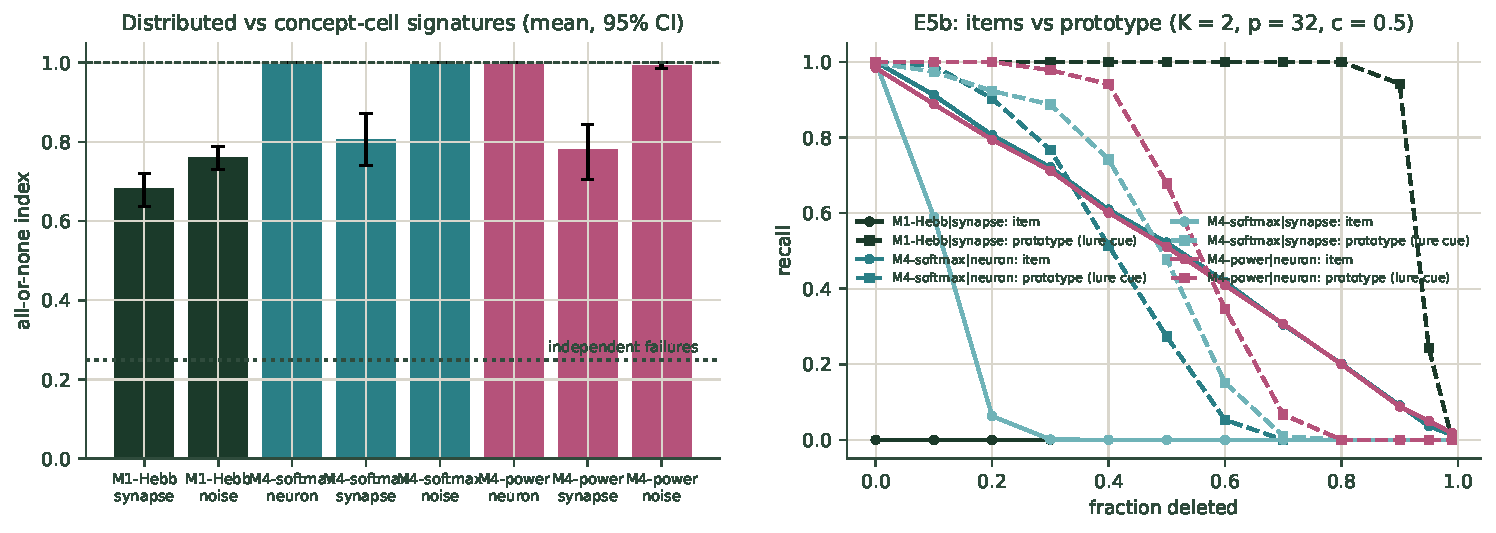
\includegraphics[width=\linewidth]{e5_aon_prototype.pdf}
\caption{E5. Top: per-memory survival curves (thin lines: the 10 memories of one network). Bottom left: all-or-none index
($1$ = each memory intact or lost; $0.25$ = independent cue-level failures). Bottom right: items vs prototype under deletion
($K=2$, $p=32$, $c=0.5$).}
\label{fig:e5}\end{figure}
Synaptic deletion in M1 degrades memories gradually and heterogeneously (AoN $0.68$ [0.64, 0.72]; weight noise $0.76$).
Deleting memory neurons in M4 removes exactly the memories whose neurons die (AoN $=1.00$ for both softmax and power).
Weight noise in M4 also acts all-or-none ($1.00$ / $0.99$), because each memory is carried by one unit's input weights.
M4 synapse deletion is intermediate ($\approx0.8$) but steep, so few sets had intermediate levels.
\textbf{Primary test (H4):} AoN, M4 neuron deletion vs M1 synapse deletion: $1.00$ vs $0.68$, paired Wilcoxon $p=1.1\times10^{-9}$. \textbf{Supported.}
\emph{Prototypes:} under synapse deletion the prototype outlasts items in M4. The level at which recall halves is 0.49 for the prototype
vs 0.12 for items (softmax), and 0.49 vs 0.11 (power). Under memory-neuron deletion it does \emph{not} for the softmax (0.41 vs 0.52) and roughly ties
for the power model (0.55 vs 0.52). However, ``gist'' (recalling some member of the right category) survives almost to total loss (0.99).
In M1 at this load only the prototype is retrievable at baseline, and it survives until $\approx92\%$ of synapses are gone.

\subsection*{E6: attention as associative memory (H5)}
\begin{figure}[H]\centering
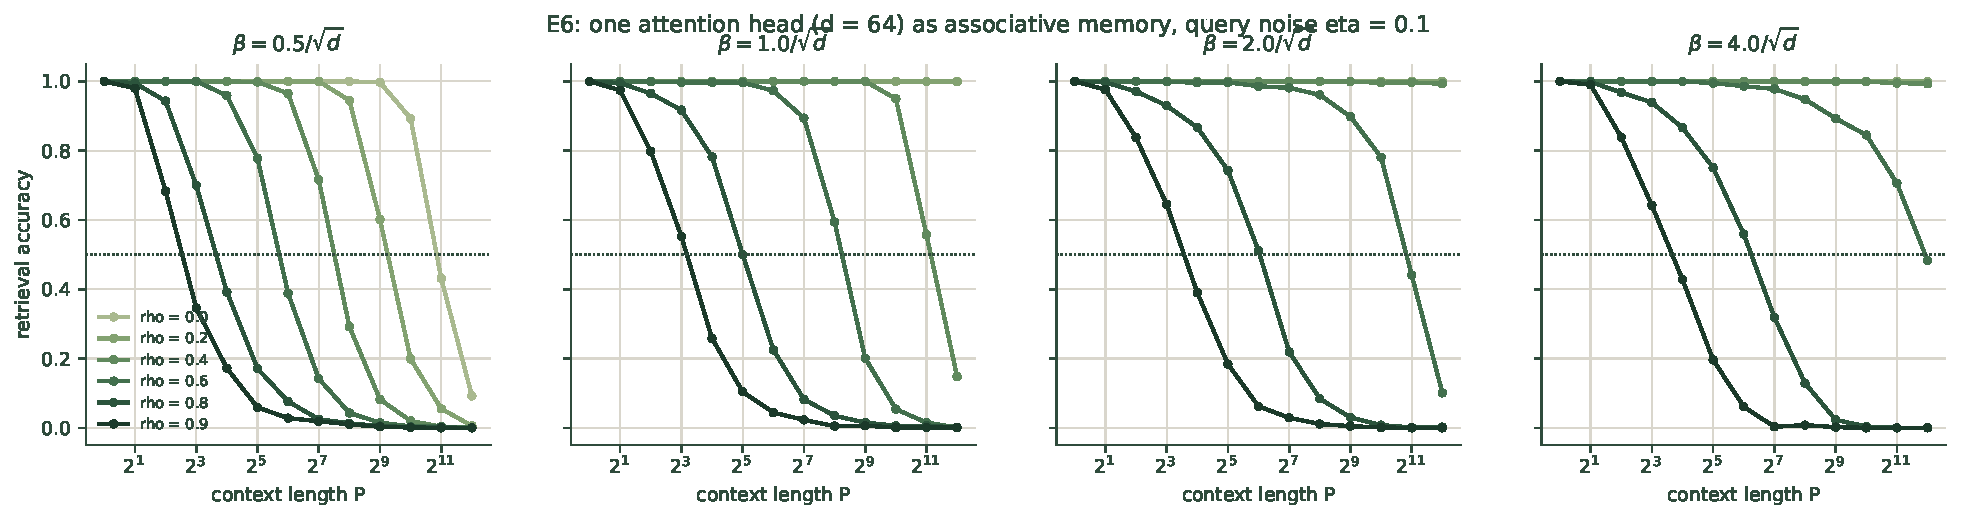
\includegraphics[width=\linewidth]{e6_accuracy.pdf}
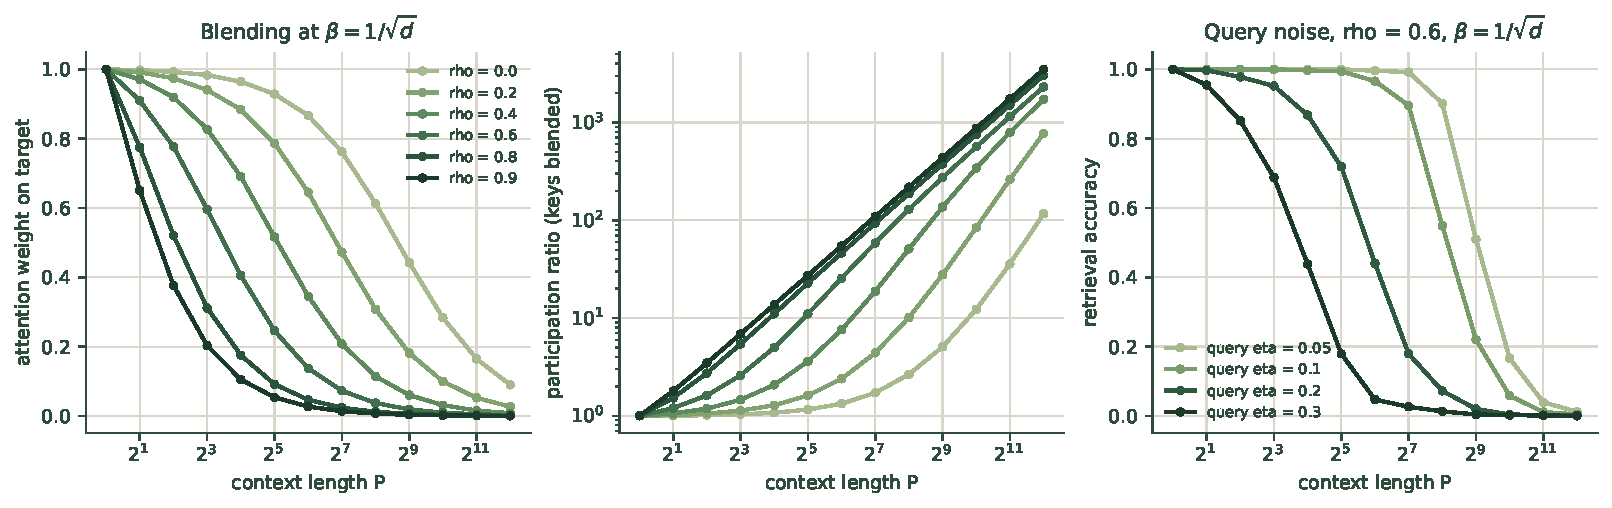
\includegraphics[width=\linewidth]{e6_blending.pdf}
\caption{E6. One attention head ($d=64$, $\beta=b/\sqrt d$): retrieval accuracy vs context length for key similarity $\rho$;
attention weight on the target and number of keys blended; query noise.}
\label{fig:e6}\end{figure}
The interference of E2/E3 appears unchanged in a single head. Accuracy falls with context length (median per-set Spearman $-0.92$ at $\rho=0.6$)
and with key similarity. At $\beta=1/\sqrt d$ the context length at 50\% accuracy is $>4096$ for $\rho\le0.2$, but $2256$, $302$, $32$ and $9$ for
$\rho=0.4,0.6,0.8,0.9$. Failures are blends: the attention weight on the target decays and the participation ratio grows, the
analogue of the low-$\beta$ blend regime. Sharper heads ($b=2,4$) tolerate longer contexts. Softer heads ($b=0.5$) fail even
for dissimilar keys ($P_{50}=1847$ at $\rho=0$).
This offers a mechanism-level account of long-context failures~\cite{liu24}, but our head has no positional structure, so it cannot reproduce the
U-shaped ``lost in the middle'' position effect itself. \textbf{Primary test (H5):} mean accuracy at $\rho=0$ vs $0.8$: $1.00$ vs $0.43$, $p=7\times10^{-10}$. \textbf{Supported.}

\subsection*{E7: forgetting and recency (H6)}
\begin{figure}[H]\centering
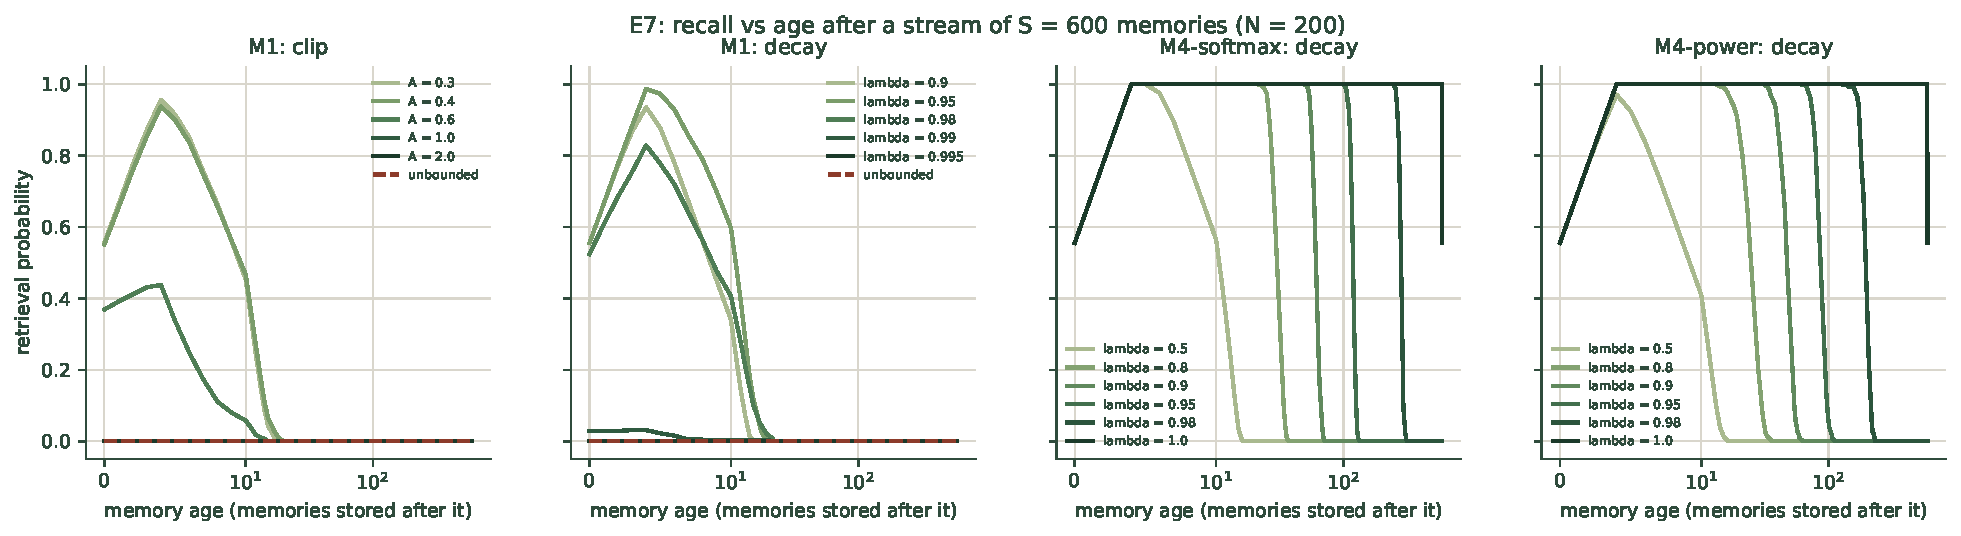
\includegraphics[width=\linewidth]{e7_recency.pdf}
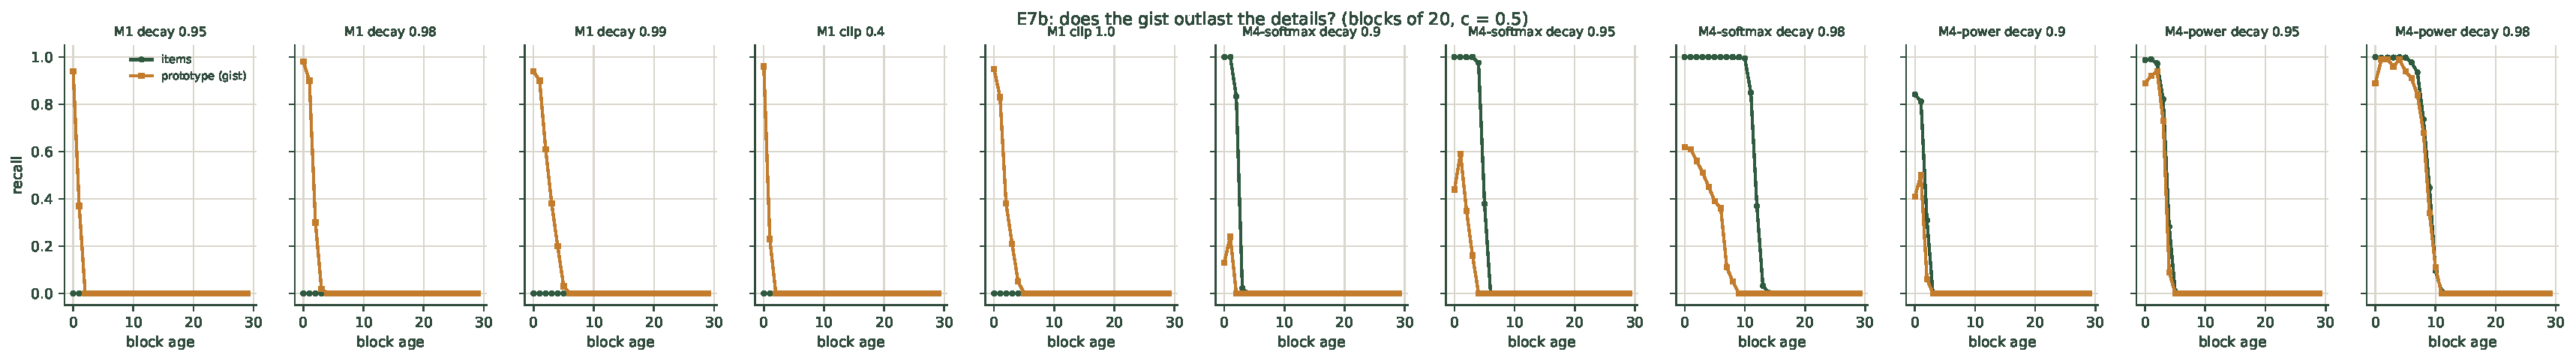
\includegraphics[width=\linewidth]{e7_gist.pdf}
\caption{E7. Top: retrieval vs memory age after a stream of $S=3N=600$ memories ($N=200$). Bottom: blocked prototype stream
(blocks of 20, $c=0.5$): item recall vs prototype (gist) recall by block age.}
\label{fig:e7}\end{figure}
The unbounded Hebbian network retrieves nothing after the stream (catastrophic blackout). Clipping ($A=0.3, 0.4$) or decay
($\lambda=0.9$--$0.98$) instead gives a recency curve with a span of 9--11 memories ($\approx0.05N$, consistent with palimpsest theory~\cite{parisi86,nadal86}).
Too loose a bound ($A\ge1$, $\lambda\ge0.99$) still blacks out, and $A=0.6$ is intermediate (span 4). In M4 the span is set by $\lambda$ and is much longer:
for softmax, 31, 61, 119 and 283 at $\lambda=0.8$, $0.9$, $0.95$ and $0.98$; for the power model, 25, 48, 87 and 197. With $\lambda=1$, all 600 memories are kept.
\textbf{Primary test (H6):} M1, the 20 most recent memories, decay $\lambda=0.98$ vs unbounded: $0.47$ vs $0.00$, $p=6\times10^{-10}$. \textbf{Supported.}
\emph{Gist:} in M1 the individual memories of a block are never retrievable, but the block's prototype is, for the last 1--3 blocks: the gist outlasts the details.
In M4 the reverse holds (softmax: item span 3--12 blocks vs prototype 0--4), and in the power model they tie. The ``prototype outlasts'' half of H6 therefore holds for the
distributed code only.

\subsection*{Optional extensions}
\begin{figure}[H]\centering
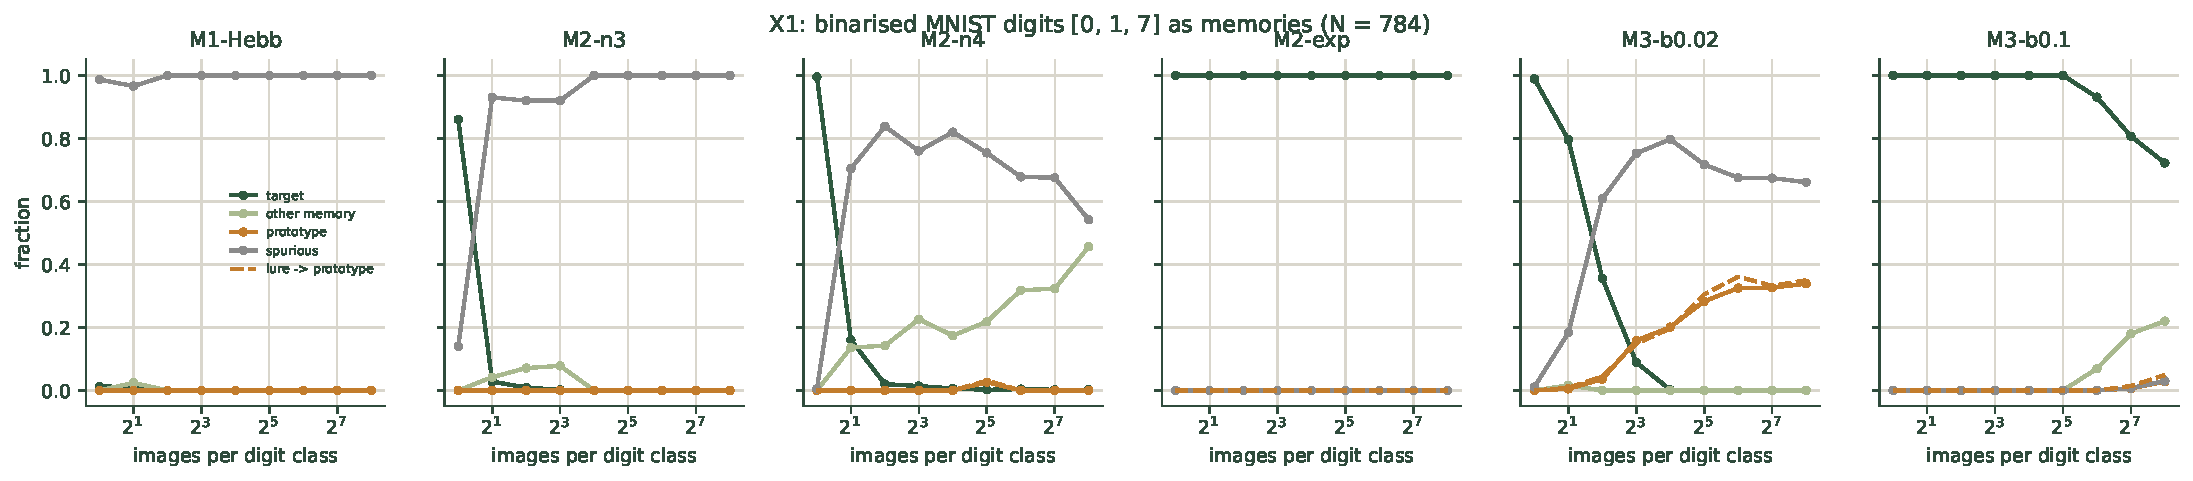
\includegraphics[width=\linewidth]{x1_mnist.pdf}
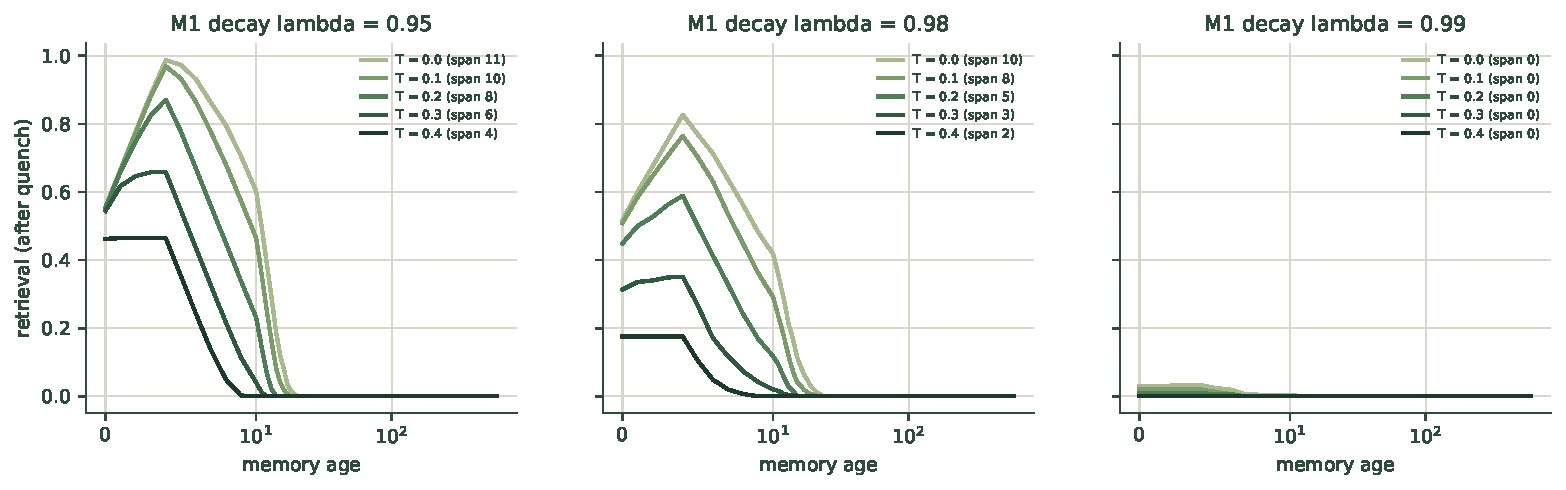
\includegraphics[width=0.75\linewidth]{x2_glauber_forgetting.pdf}
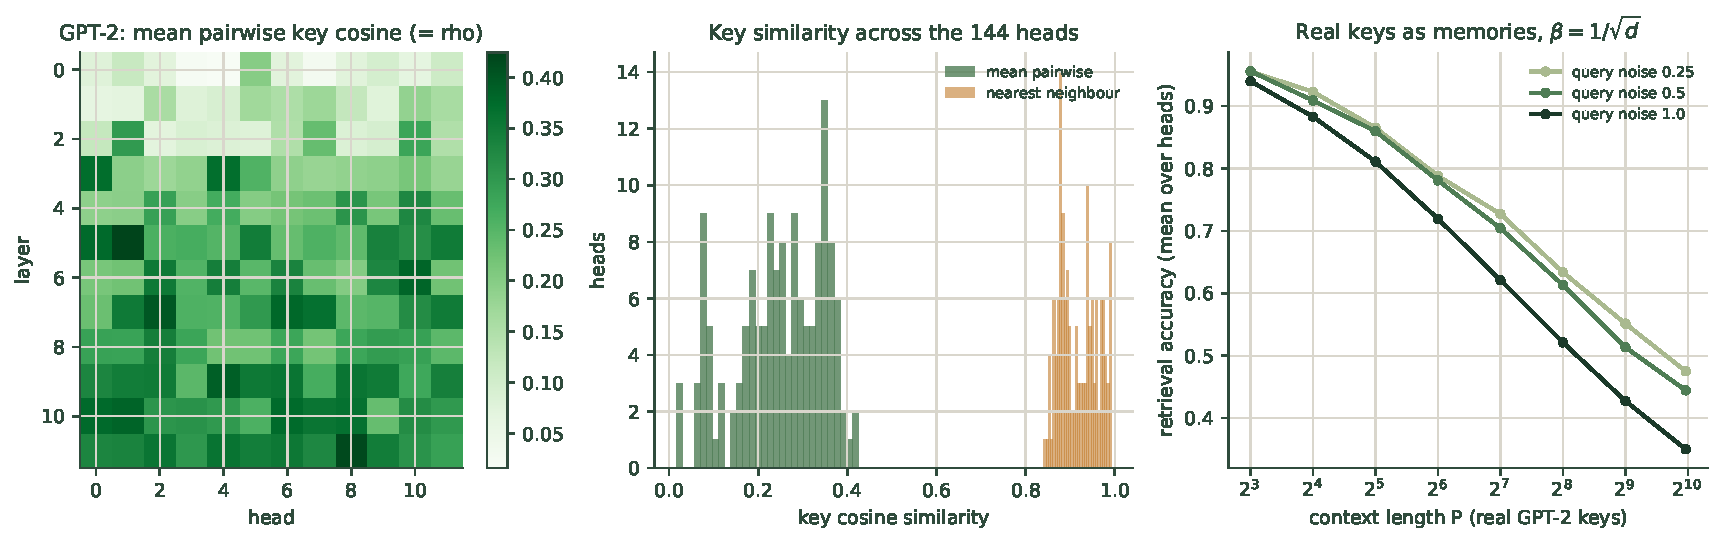
\includegraphics[width=\linewidth]{x3_gpt2.pdf}
\caption{X1: binarised MNIST digits $\{0,1,7\}$ ($N=784$). X2: Glauber noise with forgetting (M1, decay). X3: GPT-2 key similarity and retrieval with real keys.}
\label{fig:ext}\end{figure}
\textbf{X1, MNIST.} Natural digits are highly correlated: mean within-class overlap is 0.67--0.84, and overlap with the class prototype is 0.75--0.89.
M1 fails even with one image per class. $n=3$ and $n=4$ retrieve images only when one per class is stored (0.86, 1.00) and fail from two per class on. The exponential model memorises all 768 images.
M3 at $\beta=0.02$ ($\beta N\approx16$) shows the memorization$\to$generalization switch on real data: item recall falls from 0.99 to 0, and prototype
recall (from images and from lures) rises to $\approx0.35$ by 256 images per class.
\textbf{X2, noise with forgetting.} Temperature shortens the memory span monotonically (e.g.\ $\lambda=0.98$: 10, 8, 5, 3, 2 for $T=0$--$0.4$), and
noise never rescues the over-loaded $\lambda=0.99$ network.
\textbf{X3, GPT-2.} Across the 144 heads, the mean pairwise key cosine is 0.02--0.42 (median 0.26), but each key's nearest neighbour has median cosine 0.92.
Real contexts therefore contain the high-similarity distractors that E6 shows to be damaging. Using real keys as memories ($\beta=1/\sqrt d$) gives accuracy
that falls from 0.96 at $P=8$ to 0.48 at $P=1000$ (Gaussian query noise $0.25\times$ rms). Random $\pm1$ keys with a similar mean similarity ($\rho=0.2$, E6)
stay above 50\% beyond $P=4096$. The heavy tail of near-duplicate keys, not the mean similarity, drives the failures (the query-noise models differ, so this comparison is qualitative).

\subsection*{Demo}
\begin{figure}[H]\centering
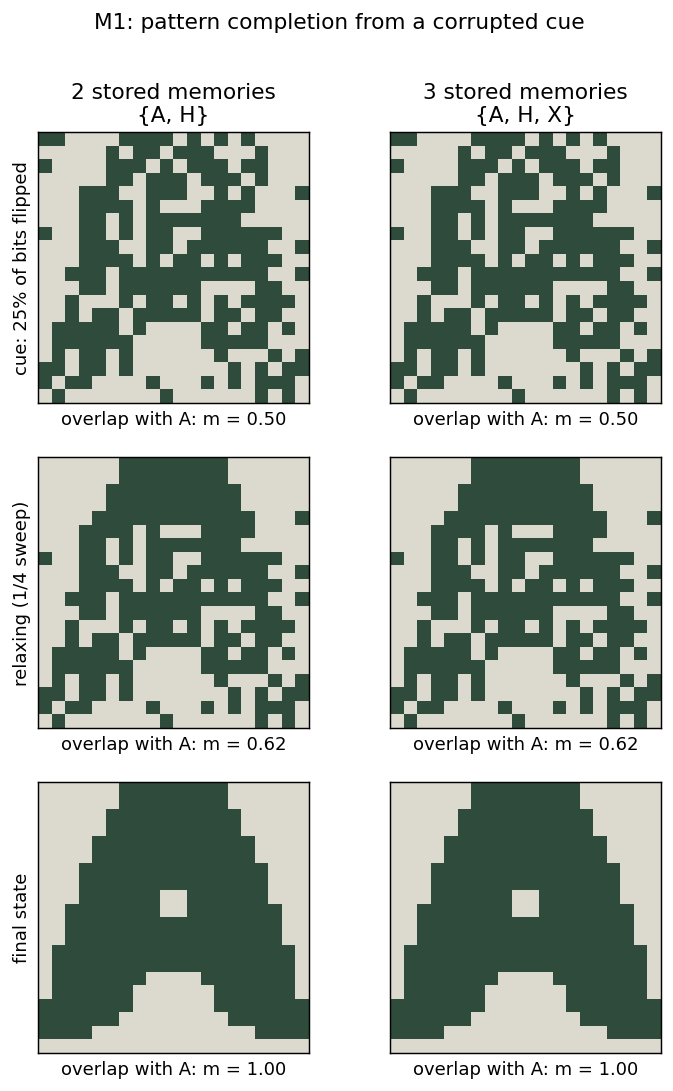
\includegraphics[width=0.30\linewidth]{recall_M1.png}\hfill
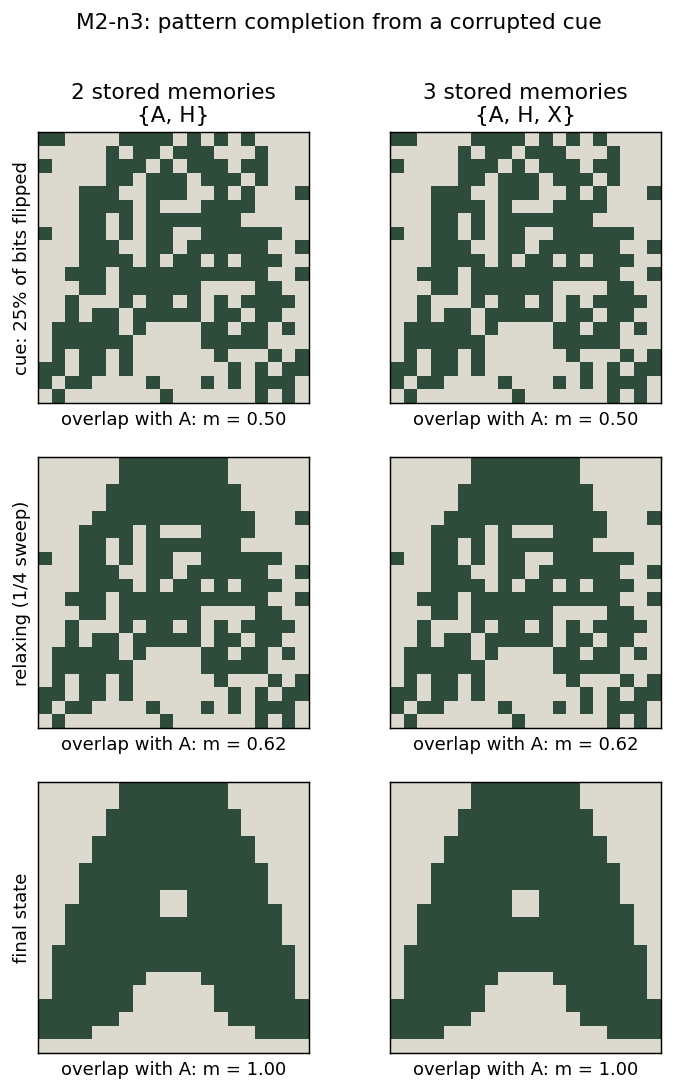
\includegraphics[width=0.30\linewidth]{recall_M2-n3.png}\hfill
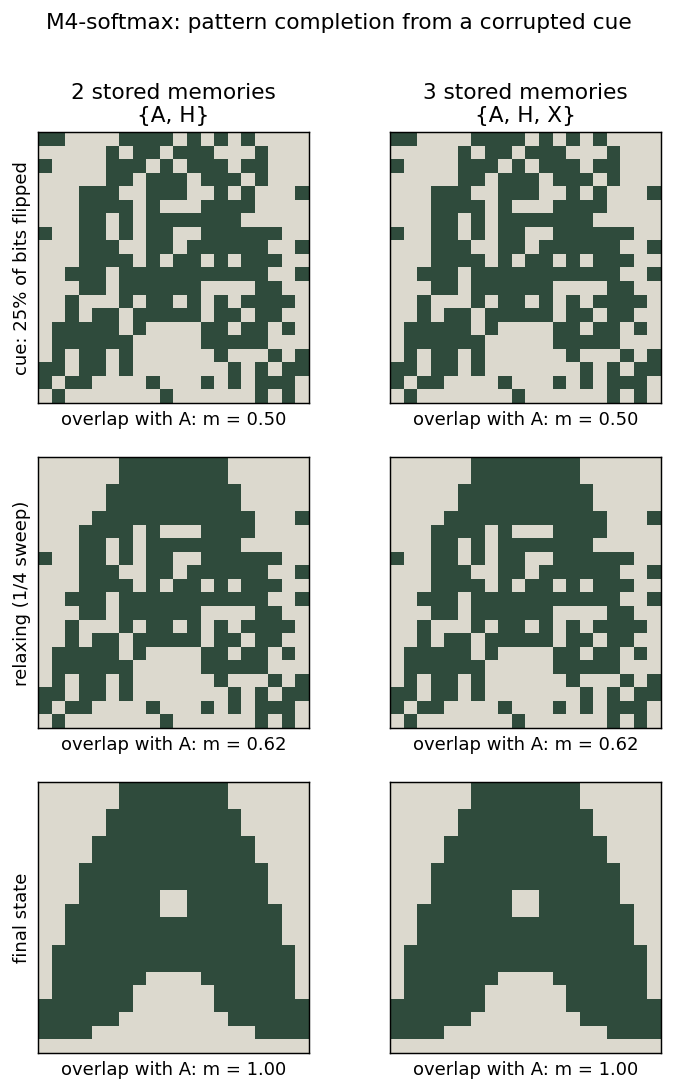
\includegraphics[width=0.30\linewidth]{recall_M4-softmax.png}
\caption{Demo (\texttt{demo/demo.py}): a cue of `A' with 25\% of bits flipped relaxes to `A' when \{A, H\} or \{A, H, X\} are stored.
Shown for M1, M2 $n=3$ and M4 (animated GIFs for all eight model variants are in \texttt{demo/out/}).}
\end{figure}

%=====================================================================
\section{Summary of hypothesis tests}
\begin{table}[H]\centering\small
\begin{tabular}{p{0.6cm}p{7.6cm}p{4.2cm}cc}\toprule
& Pre-specified primary test & Estimate & $p$ (Holm) & Verdict\\\midrule
H1 & log-log capacity slope, M2 $n=4$ minus M1 (paired bootstrap) & $2.27$ [2.23, 2.30] & $0.001$ & supported\\
H2 & $\log P^*(n=3)-\log P^*(\mathrm{M1})$, $c=0.4$ (paired bootstrap) & $1.26$ [0.87, 1.30] & $0.001$ & supported\\
H3 & per-set Spearman($\beta$, single recall), M3, $c=0.6$ (Wilcoxon) & median $0.88$ & $1\times10^{-10}$ & supported\\
H4 & all-or-none index, M4 neuron vs M1 synapse deletion (Wilcoxon) & $1.00$ vs $0.68$ & $3\times10^{-9}$ & supported\\
H5 & head accuracy, key similarity $0$ vs $0.8$ (Wilcoxon) & $1.00$ vs $0.43$ & $3\times10^{-9}$ & supported\\
H6 & recent-20 recall, M1 decay $0.98$ vs unbounded (Wilcoxon) & $0.47$ vs $0.00$ & $3\times10^{-9}$ & supported\\\bottomrule
\end{tabular}
\caption{Primary tests (50 pattern sets each). Bootstrap $p$-values are limited by resolution ($1/2000$).}
\label{tab:primary}\end{table}
\textbf{Secondary predictions not borne out (reported as found):} moderate Glauber noise did not improve retrieval near capacity (E3);
under memory-neuron deletion the prototype did not outlast individual memories in the softmax circuit (E5b); in M4 the gist did not outlast the
details under decay (E7b); the Hebbian $\alpha_c$ extrapolation brackets but does not tightly confirm 0.138 (Part A).

\section{Discussion}
One mechanism underlies all the observations: the shape of $F$ sets how sharply each memory's basin is separated from the others. Steeper $F$
(higher $n$, larger $\beta$) means higher capacity, a later switch to prototype recall, and a narrower blend regime. Softer $F$ (or noise) means
earlier generalization, false recall of lures, and gist over verbatim recall. The same quantities control a single attention head, where key similarity and context
length play the roles of $c$ and load. Representation also matters for damage and forgetting. A distributed code (M1) degrades gradually and keeps the gist.
A concept-cell code (M4) loses individual memories all-or-none and, under decay, keeps recent items rather than gists.
\textbf{Limitations.} Finite, small $N$ (exponential models only to $N=32$). Synthetic $\pm1$ patterns. The DRM and reaction-time links are analogies.
The two-layer model uses instantaneous memory neurons. E6 has no positional encoding.
\textbf{Deviations from the proposal.} Part A's load grid was extended beyond 0.30 (to 0.60) so that the Storkey crossing could be measured. E1 used $\eta=0.125$ with $N$
a multiple of 8 so that corruption is identical across $N$. E5a used 4 cues per memory (40 per set) to measure per-memory survival.
Runs were executed on Kaggle CPU kernels rather than locally. All other parameters follow the proposal.

\paragraph{Reproducibility.} \texttt{./run\_all.sh} (or \texttt{QUICK=1} for a smoke test) regenerates every number and figure from the master seed;
the code, raw results (\texttt{results/}) and figures are in the repository.

\appendix
\section{Additional figures}
\begin{figure}[H]\centering
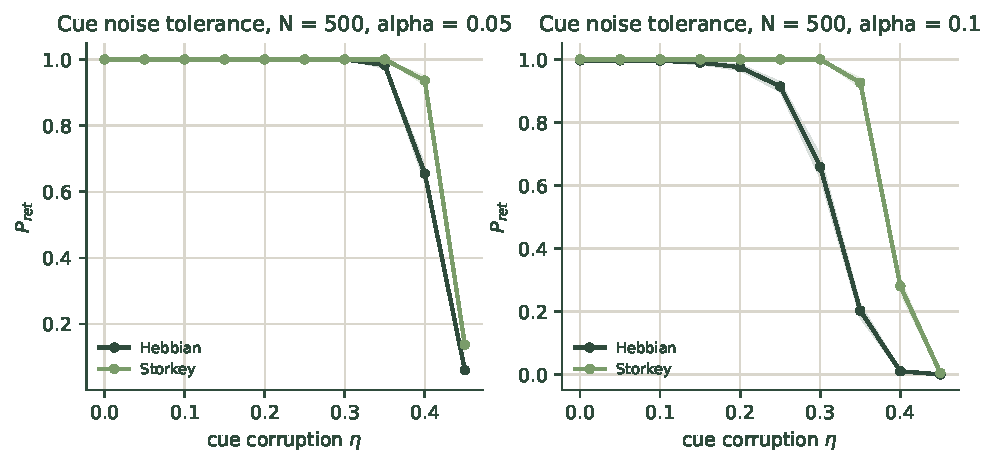
\includegraphics[width=0.7\linewidth]{partA_cue_noise.pdf}
\caption{Part A. Cue-noise tolerance, $N=500$ ($\eta_{50}$ in the text).}
\end{figure}
\begin{figure}[H]\centering
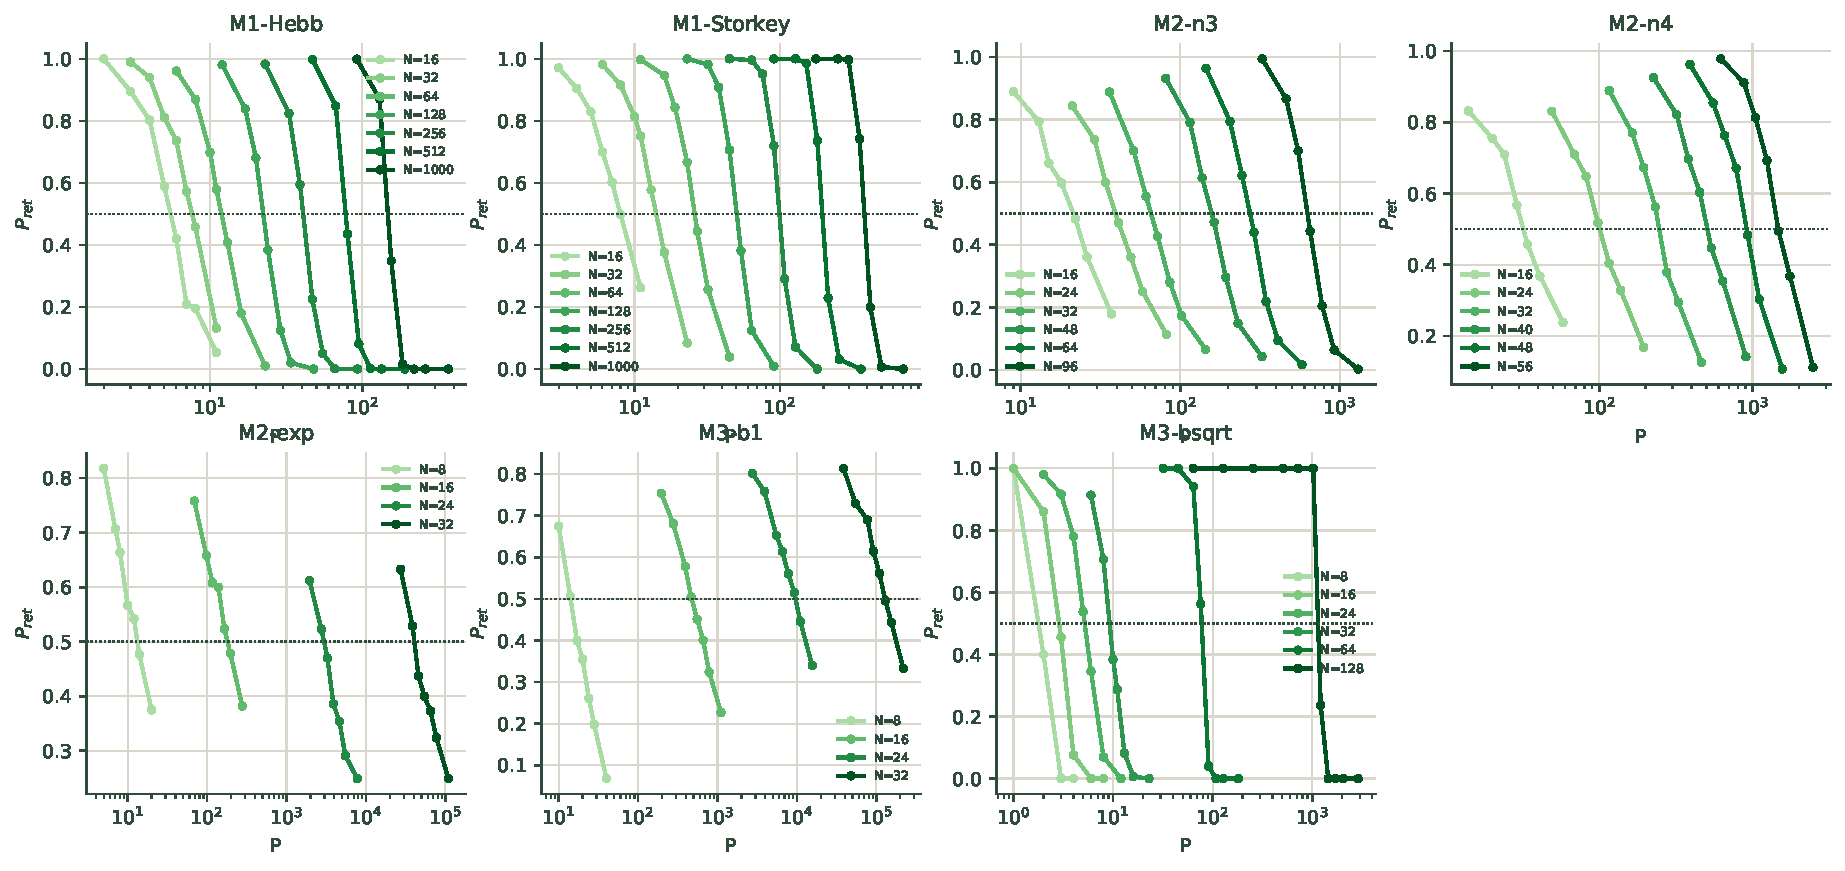
\includegraphics[width=\linewidth]{e1_retrieval_curves.pdf}
\caption{E1. Retrieval probability vs $P$ for every model and $N$ (adaptive ladder points; dotted: 0.5).}
\end{figure}

\begin{thebibliography}{99}\small
\bibitem{hopfield82} J.~J. Hopfield. Neural networks and physical systems with emergent collective computational abilities. \emph{PNAS} 79(8):2554--2558, 1982.
\bibitem{amit85} D.~J. Amit, H.~Gutfreund, H.~Sompolinsky. Storing infinite numbers of patterns in a spin-glass model of neural networks. \emph{PRL} 55(14):1530--1533, 1985.
\bibitem{fontanari90} J.~F. Fontanari. Generalization in a Hopfield network. \emph{J. Physique} 51(21):2421--2430, 1990.
\bibitem{krotov16} D.~Krotov, J.~J. Hopfield. Dense associative memory for pattern recognition. NeurIPS 29, 2016.
\bibitem{demircigil17} M.~Demircigil, J.~Heusel, M.~L\"owe, S.~Upgang, F.~Vermet. On a model of associative memory with huge storage capacity. \emph{J. Stat. Phys.} 168:288--299, 2017.
\bibitem{ramsauer21} H.~Ramsauer et al. Hopfield networks is all you need. ICLR, 2021.
\bibitem{krotov21} D.~Krotov, J.~J. Hopfield. Large associative memory problem in neurobiology and machine learning. ICLR, 2021.
\bibitem{kozachkov25} L.~Kozachkov, J.-J. Slotine, D.~Krotov. Neuron-astrocyte associative memory. \emph{PNAS} 122(21):e2417788122, 2025.
\bibitem{ambrogioni24} L.~Ambrogioni. In search of dispersed memories: Generative diffusion models are associative memory networks. \emph{Entropy} 26(5):381, 2024.
\bibitem{pham25} B.~Pham, G.~Raya, M.~Negri, M.~J. Zaki, L.~Ambrogioni, D.~Krotov. Memorization to generalization: Emergence of diffusion models from associative memory. arXiv, 2025.
\bibitem{krotov23} D.~Krotov. A new frontier for Hopfield networks. \emph{Nat. Rev. Phys.} 5:366--367, 2023.
\bibitem{roediger95} H.~L. Roediger, K.~B. McDermott. Creating false memories. \emph{J. Exp. Psychol. LMC} 21(4):803--814, 1995.
\bibitem{quiroga05} R.~Quian Quiroga, L.~Reddy, G.~Kreiman, C.~Koch, I.~Fried. Invariant visual representation by single neurons in the human brain. \emph{Nature} 435:1102--1107, 2005.
\bibitem{amit87} D.~J. Amit, H.~Gutfreund, H.~Sompolinsky. Statistical mechanics of neural networks near saturation. \emph{Ann. Phys.} 173(1):30--67, 1987.
\bibitem{storkey97} A.~Storkey. Increasing the capacity of a Hopfield network without sacrificing functionality. ICANN '97, LNCS 1327:451--456, 1997.
\bibitem{parisi86} G.~Parisi. A memory which forgets. \emph{J. Phys. A} 19(10):L617--L620, 1986.
\bibitem{nadal86} J.-P. Nadal, G.~Toulouse, J.-P. Changeux, S.~Dehaene. Networks of formal neurons and memory palimpsests. \emph{Europhys. Lett.} 1(10):535--542, 1986.
\bibitem{mezard86} M.~M\'ezard, J.-P. Nadal, G.~Toulouse. Solvable models of working memories. \emph{J. Physique} 47(9):1457--1462, 1986.
\bibitem{lucibello24} C.~Lucibello, M.~M\'ezard. The exponential capacity of dense associative memories. \emph{PRL} 132:077301, 2024.
\bibitem{liu24} N.~F. Liu et al. Lost in the middle: How language models use long contexts. \emph{TACL} 12:157--173, 2024.
\bibitem{glauber63} R.~J. Glauber. Time-dependent statistics of the Ising model. \emph{J. Math. Phys.} 4(2):294--307, 1963.
\bibitem{robinson97} K.~J. Robinson, H.~L. Roediger. Associative processes in false recall and false recognition. \emph{Psychol. Sci.} 8(3):231--237, 1997.
\end{thebibliography}
\end{document}
